% !TEX root = ../main.tex

\chapter{An Introduction to Bayesian Inference}
\label{chp:inf}

% !TEX root = ../main.tex

\section{The Challenge of Bayesian Inference}
\label{sec:inf:challenge}

In the previous chapter we introduced the concept of Bayesian modelling and showed how we
can combine prior information $p(\theta)$ and a likelihood model $p(\mathcal{D}|\theta)$ using Bayes' rule 
(i.e.~\eqref{eq:bayes}), to produce a posterior $p(\theta|\mathcal{D})$ on variables $\theta$ that
characterizes both our prior information and information from the data $\mathcal{D}$.  We now consider the
problem of how to calculate (or more typically approximate) this posterior, a process 
known as Bayesian \emph{inference}.
At first this may seem like a straight forward problem: by Bayes' rule we have that
$p(\theta|\mathcal{D})\propto p(\mathcal{D}|\theta)p(\theta)$ and so we already know the relative probability of any one
value of $\theta$ compared to another.  In practice, this could hardly be further from the
truth.  Bayesian inference for the general class of graphical models is in fact an 
NP-hard problem \citep{cooper1990computational,dagum1993approximating}.  We can break
it down into key challenges: calculating the normalization constant
$p(\mathcal{D}) = \int p(\mathcal{D}|\theta)p(\theta)d\theta$ and providing a useful characterization of the posterior, for
example an object we can draw samples from.  Many inference schemes, for example Markov
chain Monte Carlo (MCMC) methods \citep{hastings1970monte}, will not
try to tackle these challenges directly and instead look to generate samples directly from 
the posterior.  However, this breakdown will still prove useful in illustrating the intuitions
about the difficulties presented by Bayesian inference.

\subsection{The Normalization Constant}
\label{sec:inf:challenge:norm}

Calculating the normalization constant in Bayesian inference is essentially a problem of
integration.  Our target, $p(\mathcal{D})$, is the expectation of the likelihood under the prior,
hence the name \emph{marginal likelihood}.  When $p(\mathcal{D})$ is known, the posterior can be evaluated
exactly at any possible input point using~\eqref{eq:bayes} directly.  When it is unknown, we lack
a scaling in the evaluation of any point and so we have no concept of how relatively 
significant that point is relative to the distribution as a whole.  For example, for a discrete
problem then if we know the normalizing constant, we can evaluate the exact probability of any
particular $\theta$ by evaluating that point alone.  If we do not know the normalizing constant, we do
not know if there are other substantially more probable events that we have thus-far missed, which
would in turn imply that the queried point has a negligible chance of occurring.
 
To give a more explicit example, consider a model where $\theta \in \{1,2,3\}$ with a corresponding uniform prior $P(\theta) = 1/3$
for each $\theta$.  Now presume that for some reason that we are only able to evaluate the likelihood at 
$\theta=1$ and $\theta=2$, giving $p(\mathcal{D}|\theta=1)=1$ and $p(\mathcal{D}|\theta=2)=10$ respectively.  Depending on the marginal
likelihood $p(\mathcal{D})$, the posterior probability of $P(\theta=2 | \mathcal{D})$ will vary wildly.  For example,
$p(\mathcal{D})=4$ gives $P(\theta=2 | \mathcal{D}) = 5/6$, while $p(\mathcal{D})=1000$ gives $P(\theta=2 | \mathcal{D}) = 1/100$.  Though this
example may seem far-fetched, this is the scenario almost always seen in practice for realistic
models, at least those with non-trivial solutions.   Typically it is not
possible to enumerate all the possible values of $\theta$ in reasonable time and we are left 
wondering - how much probability mass is left that we have not seen?  The problem is even worse 
in the setting where $\theta$ is continuous, for
which it is naturally impossible to evaluate all possible values for $\theta$.  
Knowing the posterior only up to a normalization constant is deceptively unhelpful - we never
know how much of the probability mass we have missed and therefore whether the probability (or
probability density) where we have looked so far is tiny compared to some other dominant region
we are yet to explore.  At its heart, the problem of Bayesian inference is a problem
of where to concentrate our finite computational resources so that we can effectively characterize
the posterior.  If $p(\mathcal{D})$ is known, then we immediately know whether we are looking in the right
place or whether there are places left to look that we are yet to find.  This brings us onto
our second challenge - knowing the posterior in closed form is often not enough.

\todo[inline]{Maybe talk about things in terms of the explore-exploit dilema a bit?}

\subsection{Characterizing the Posterior}
\label{sec:inf:challenge:post}

Once with have the normalization constant, it might seem that we are done; after all
we now have the exact form the posterior using in Bayes' rule.  Unfortunately, it tends to
be the case, at least when $\theta$ is continuous, that is this insufficient to carry out most
tasks that we might want to use our posterior for.  There are a number of different, often
overlapping, reasons for wanting to calculate a posterior including
\begin{itemize}
	\item To calculate the posterior probability or probability density for one or more particular
	instances of the variables.
	\item To calculate the expected value of some function, $\mu_f = \E_{p(\theta|\mathcal{D})}\left[f(\theta)\right]$.
	For example, we might want to calculate the expected values of the variables themselves
	$\mu_\theta = E_{p(\theta|\mathcal{D})} \left[\theta\right]$ as a point estimate.
	\item To make predictions.  For example, in a supervised learning task then our data typically
	comprises of a series of input output pairs $\mathcal{D} = \{x_n,y_n\}_{n=1:N}$ and we
	wish to predict the output at some new input $\tilde{x}$.  In the fully Bayesian framework, one
	does this using the \emph{posterior predictive distribution}
	\[
	p(\tilde{y} | \tilde{x}) = \int p(\tilde{y}|\tilde{x},\theta) p(\theta | \mathcal{D}) d\theta.
	\]
	Note that this is a particular case of calculating an expectation under the posterior.
	\item To find the most probable variable values $\theta^* = \argmax_{\theta} p(\theta|\mathcal{D})$.  
	This is known
	as maximum a posteriori estimation and will be discussed in Chapter~\ref{chp:opt}.
	\item To produce samples from, or form some other useful characterization of, the posterior that can
	then passed on to another part of a computational pipeline or directly observed by a user.
	\item To estimate a marginal probability distribution over some variables of particular
	interest.  For example, if $\theta=\{u,v\}$ then we might be interest in the marginal
	$p(u|\mathcal{D})$.
\end{itemize}
If $\theta$ is continuous or some elements of $\theta$ are continuous then only the first of
these can be carried out directly using the form of the posterior provided by Bayes' rule
with known normalization constant.  We, therefore, see that knowing the normalization alone
will not be enough to fully solve the Bayesian inference problem in a useful manner.  In
particular, it will generally not sufficient in order to be able to \emph{sample} from the
posterior.  As we will see later, the ability to sample will be at the core of most practical uses
for the posterior as it allows use of Monte Carlo
 methods~\citep{metropolis1949monte,robert2004monte,rubinstein2016simulation}, which
 can in turn be used to carry out many of the outlined tasks.

To further demonstrate why knowing the normalization constant is insufficient
for most Bayesian inference tasks, we consider a simple example.  
% !TEX root = ../main.tex

\section{Monte Carlo}
\label{sec:inf:mc}

Monte Carlo~\citep{metropolis1949monte} is the characterization of a probability distribution 
through random sampling. It is the foundation for a huge array of methods for numerical 
integration, optimization, and scientific simulation; forming the underlying principle 
for all stochastic computation.
\mc provides us with a means of dealing with complex models and problems in a
statistically principled manner.  Without it, one would have to resort to deterministic
approximation methods whenever the target problem is too complex to permit analytic
solution.  As we will show, it is a highly composable framework that will allow to output
of one system to be input directly to another.  For example, the \mc samples from a joint
distribution will also have the correct marginal distribution over any of its individual components,
while sampling from the marginal distribution then sampling from the conditional distribution
given these samples will give samples distributed according to the joint.  As \mc
will be key to most methods for Bayesian inference that we will consider, we take the time
in this section to introduce Monte Carlo at a foundational level.

The most common usage of \mc in this work will be the \mc estimation of expectations, 
sometimes known as \mc integration.  
The critical importance of \mc estimation stems from the fact that most of the example
target tasks laid out in~\ref{sec:inf:challenge:post} can be formulated as expectations.
Even when our intention is simply to generate samples from a target distribution, we can
usually think of this as being an implicit expectation of an, as-yet unknown, target function.
Here our implicit aim is to minimize the bias and variance of whatever process the samples are eventually
used for, even if that process is simply visual inspection.  

Consider the problem of calculating the expectation of some function
$f(\theta)$ under the distribution $\theta\sim \pi(\theta)$ ($= p(\theta | \mathcal{D})$ for the Bayesian
inference case), which we will denote 
as
\begin{align}
	\label{eq:inf:expt}
I:=\E_{\pi(\theta)} \left[f(\theta)\right]=\int f(\theta) \pi(\theta) d\theta.
\end{align}
This can be approximated using the \mc estimator $I_N$ where
\begin{align}
	\label{eq:inf:mc-est}
	I \approx I_N := \frac{1}{N} \sum_{n=1}^{N}f(\hat{\theta}_n)
	\quad \text{where} \quad \hat{\theta}_n \sim \pi(\theta).
\end{align}
The first result we note is that~\eqref{eq:inf:mc-est} is an \emph{unbiased} estimator for $I$, i.e. we have
\begin{align}
\label{eq:inf:unbiased}
\E \left[I_N\right] = \E \left[\frac{1}{N} \sum_{n=1}^{N}f(\hat{\theta}_n)\right]
= \frac{1}{N} \sum_{n=1}^{N} \E \left[f(\hat{\theta}_n)\right]
= \frac{1}{N} \sum_{n=1}^{N} \E \left[f(\hat{\theta}_1)\right]
= I
\end{align}
where we have first moved the sum outside of expectation using
linearity,\footnote{Note that this presumes that $N$ is independent
	of the samples.  This is usually the case, but care is necessary in some situations, namely when
	the number of samples taken is adaptively chosen based on the sample values, for example in
	adaptive stratified sampling~\citep{etore2010adaptive}.}
then the fact that each $\hat{\theta}_n$ is identically distributed to note that
each $\E \left[f(\hat{\theta}_n)\right]= \E \left[f(\hat{\theta}_1)\right]$, and finally
that $\E \left[f(\hat{\theta}_1)\right] = I$ by the definition of $I$ and the distribution
on $\hth_1$.  This is an important result as it means that \mc does not introduce
any systematic error, i.e. bias, into the approximation: in expectation it does not
pathologically overestimate or underestimate the target.  This is not to say though that it is
equally likely to overestimate or underestimate as it may, for example, typically underestimate
by a small amount and then rarely overestimate by a large amount.  Instead, it means that if we
were to repeat the estimation an infinite number of times and average the results, we would
get the true value of $I$.  This now hints at another important question -- do we also get
recover the true value of $I$ when we conduct one infinitely large estimation, namely if we
take $N\rightarrow\infty$?  This is known as \emph{consistency} of a statistical estimator,
which we will now consider next.  Before moving
on, we make the important note that many common \mc inference methods, for example MCMC, are in fact biased.  
This is because it is often not possible to sample $\hth_n \sim \pi(\theta)$
exactly as we have assumed in~\eqref{eq:inf:mc-est}, with the bias resulting from
the approximation.  The convergence of such methods relies on the bias 
diminishing to $0$ as $N\rightarrow\infty$, such that they remain unbiased in the limit.

\subsection{The Law of Large Numbers}
\label{sec:inf:mc:law}

A key mathematical idea underpinning the convergence of many Monte Carlo methods is the 
law of large numbers (LLN).  Informally, the LLN states that the empirical average of 
independent and identically distributed (i.i.d.)  random variables converges to 
the true expected value of the underlying process as the number of samples in the
average increases.  We can there use it to prove the consistency of Monte Carlo estimators
where the samples are drawn independently from the same distribution, as is the case
in for example rejection sampling and importance sampling.  The high level idea for the LLN can be shown by
considering the  \emph{mean squared error} of a \mc estimator as 
follows
%\footnote{Note here that we use the notation of expectation typically used within the statistics literature,
%whereby it corresponds to the expectation over all randomness contained in the system.}
\begin{align}
\E &\left[(I_N-I)^2\right] = \E\left[\left(\frac{1}{N}\sum_{n=1}^{N}f(\hth_n) - I\right)^2\right] \nonumber \\
&= \frac{1}{N^2}\sum_{n=1}^{N} \E\left[ \left(f(\hth_n)-I\right)^2\right] + 
\frac{1}{N(N-1)}\sum_{n=1}^{N}\sum_{m=1,m\neq n}^{N} \E\left[ (f(\hth_n)-I)(f(\hth_m)-I)\right] \nonumber \\
&= \frac{1}{N^2}\sum_{n=1}^{N} \E\left[ \left(f(\hth_1)-I\right)^2\right] + 
\frac{1}{N(N-1)}\sum_{n=1}^{N}\sum_{m=1,m\neq n}^{N} \cancelto{0}{\left(\E\left[(f(\hth_1)-I)\right]\right)^2} \nonumber \\
&= \frac{\sigma_{\theta}^2}{N}  \quad \text{where} \quad \sigma_{\theta}^2 := \E\left[ \left(f(\hth_1)-I\right)^2\right]
= \var \left[f(\theta)\right].\label{eq:inf:LLN-informal}
\end{align}
Here the second line follows from the first simply by expanding the square and using linearity
to move the sum outside of the expectation as in the unbiasedness derivation.
The first term in the third line follows from the equivalent term in the second line by again noting that
each $\hth_n$ has the same distribution.  The second term in the third line
follows from the assumption that the samples are drawn independently such that
\[
\E\left[ (f(\hth_n)-I)(f(\hth_m)-I)\right] = \E\left[ (f(\hth_n)-I)\right] \E\left[(f(\hth_m)-I)\right]=0.
\]
by unbiasedness of the estimator. The last line simply notes that $\E\left[ \left(f(\hth_1)-I\right)^2\right]$ is a constant,
namely the variance of $f(\theta)$.
  Our final result has a simple and intuitive form -- the mean squared error for
our estimator using $N$ samples, is $1/N$ times the mean squared error of an estimator that only uses
a single sample, which is itself equal to the variance of $f(\theta)$.  As $N\rightarrow\infty$, we thus
have that our expected error goes to $0$.

A key upshot of this result is that the difference between our empirical estimate and the true value (i.e. $I_N-I$)
 should be of order $O(1/\sqrt{N})$.  In some way this is rather slow: deterministic numerical
integration schemes of have much fast convergence theoretical convergence rates.  For example,
Simpson's rule has a a convergence rate of $O(1/n^4)$ for one dimensional functions.  
As such, \mc is often an inferior way of estimating integrals for smooth functions
in low dimensions.  However, this
requires smoothness assumptions on $f$ and, more critically, the convergence rate diminishes rapidly
in higher dimensions.   
The dimensionality only effects the \mc convergence rate through changes in the constant factor $\sigma_{\theta}$
and though this will typically increase with the dimensionality, this 
scaling will typically be substantially more graceful than deterministic numerical methods.
%generally do so substantially less aggressively
%then typical exponential decrease in converge rate of deterministic numerical integration schemes
%with dimension.  
%\mc therefore tends to dominate for moderate to high dimensional problems.

\subsection{Convergence of Random Variables}
\label{sec:inf:mc:conv}

To introduce the concept the LLN more precisely, we now consider some more formal notations
of convergence of random variables.  There will be times (e.g. Chapter~\ref{chp:nest})
when mathematical rigour will require us to distinguish between alternative notations of convergence.
However, those less interested in theoretical details may wish to
skip Sections~\ref{sec:inf:mc:conv:prob},~\ref{sec:inf:mc:conv:as}, and~\ref{sec:inf:mc:conv:dist}
on first reading, as the notion of $L^p$ convergence will be sufficient, for most practical purposes,
to guarantee that an estimator will return the correct answer if provided 
with sufficient samples. 

\subsubsection{$L^p$-Convergence}
\label{sec:inf:mc:conv:Lr}

We start by introducing the notion of $L^p$-convergence, also known as convergence in expectation,
as this is the type of convergence we have just alluded to in our informal proof of the LLN.
At a high level, $L^p$-convergence means that the expected value of the related error metric
tends to zero as $N\rightarrow \infty$.  More precisely, we first define the $L^p$-norm for
a random variable $X$ as
\begin{align}
\label{eq:inf:Lp-norm}
\norm{X}_p = \left(\E \left[\left|X\right|^{p}\right]\right)^{\frac{1}{p}}
\end{align}
where $\left|\cdot\right|$ denotes the absolute value.  For example, we can write the
mean squared error used in~\eqref{eq:inf:LLN-informal} as the squared $L^2$-norm:
$\E \left[(I_N-I)^2\right] = \norm{I_N-I}_2^2$.  We further define the notion of $L^p$-space
as being the space of random variables for which $\norm{X}_p < \infty$.  We can now
formally define $L^p$-convergence as follow.
\begin{definition}[$L^p$-convergence]
A sequence of random variables $X_N$ converges in its $L^p$-norm to 
$X$ (where $p\ge1$) if $X\in L^p$, each $X_N \in L^p$, and
\begin{align}
\lim\limits_{N\rightarrow\infty} \norm{X_N-X}_p=0. \label{eq:inf:Lp-conv-formal}
\end{align}
\end{definition}
\noindent A key point to note is that $\Vert X_N-X\rVert_p\ge0 \; \forall X_N, X$ by definition of the $L^p$-norm and so
rather than this simply being a statement of asymptotic unbiasedness, $L^p$-convergence says that the expected
\emph{magnitude} of the error tends to zero as $N\rightarrow\infty$.
Different values of $p$ correspond to different metrics for the error, with larger values of
$p$ constituting stronger converge guarantees, such that $L^{p_2}$-convergence implies
$L^{p_1}$-convergence whenever $p_2>p_1$.  Similarly, if a a random variable satisfies
$X \in L^{p_2}$, then it follows that $X \in L^{p_1}$.

%
%\subsubsection{Convergence in Distribution}
%\label{sec:inf:mc:conv:dist}
%
%Convergence in distribution is a weaker form of convergence than is implied by all the
%other forms of convergence that we will discuss.

\subsubsection{Convergence in Probability}
\label{sec:inf:mc:conv:prob}

At a high level, convergence in probability between two random variables (or between a random variable and
a constant) means that they become arbitrary close to one another.  More
formally we have the following definition.
\begin{definition}[Convergence in probability]
A sequence of random variables $X_N$ converges in probability to $X$ if, for every $\varepsilon>0$,
\begin{align}
\lim\limits_{N\rightarrow\infty} P(\left|X_N-X\right|\ge\varepsilon)=0.
\end{align}
\end{definition}
\noindent As $\varepsilon$ can be made arbitrarily small, this ensures that $X_N$ becomes arbitrarily
close to $X$ in the limit of large $N$.  Estimators are \emph{consistent} if they converge
in probability.

In~\eqref{eq:inf:LLN-informal} we demonstrated the $L^2$ convergence of the Monte Carlo
estimator as we have that 
\[
\lim\limits_{N\rightarrow\infty} \norm{I_N-I}_2=\lim\limits_{N\rightarrow\infty} \frac{\sigma_\theta}{\sqrt{N}} = 0.
\]
Convergence in probability is, in general, a weaker form of convergence than $L^p$ convergence
as $L^p$ convergence implies convergence in probability~\citep{williams1991probability}.
We therefore also have the Monte Carlo estimator convergences in
probability to its expectation.  This is known as the
\emph{weak law of large numbers}, which we can also prove more explicitly as follows
\begin{theorem}[Weak law of large numbers]
	\label{the:inf:weak-law}
If $I$ and $I_N$ are defined as per~\eqref{eq:inf:expt} and~\eqref{eq:inf:mc-est} respectively,
$I\in L^1$, each $I_N \in L^1$,
 and each $\hth_n$ in~\eqref{eq:inf:mc-est} is drawn independently, then $I_N$ converges to $I$
in probability:
	$\lim\limits_{N\rightarrow\infty} P(\left|I_N-I\right|\ge \varepsilon)=0 \quad \forall \varepsilon>0$.
\end{theorem}
\begin{proof}
In the interest of exposition, we prove the result in the case where the stronger 
assumptions that $I\in L^2$ and each $I_N \in L^2$ hold.  In practise this is not needed as
the theorem can be proved by other means, see for example~\cite[Theorem 2.2.7]{durrett2010probability}.

By~\eqref{eq:inf:unbiased} we have that $\E [I_N]=I$ and by~\eqref{eq:inf:LLN-informal} we have that 
$\norm{I_N-I}_2^2 = \frac{\sigma_{\theta}^2}{N}$
where $\sigma_{\theta}^2$ is an unknown, but finite, constant by the assumption that $I\in L^2$.
Chebyshev's inequality states that if $\E [I_N] = I$, then for any $k>0$
\[
P(\left|I_N-I\right|\ge\varepsilon)\le\frac{\var(I_N)}{\varepsilon^2}.
\]
By further noting that as $I_N$ is unbiased, we have that $\var(I_N) = \norm{I_N-I}_2^2$
and therefore
\[
\lim\limits_{N\rightarrow\infty} P(\left|I_N-I\right|\ge\varepsilon)
\le\lim\limits_{N\rightarrow\infty} \frac{\sigma_{\theta}^2}{\varepsilon^2 N}
=0 \quad \forall \varepsilon>0.
\]
\end{proof}
%\noindent As an interesting aside, we can prove that convergence in probability follows from
%$L^p$ convergence more generally in a similar fashion.  This can be done
%by using the more general form of Chebyshev's inequality given in, for example,
%Theorem 1.6.4 and Lemma 2.2.2 of~\cite{durrett2010probability} to show that
%\begin{align}
%\label{eq:inf:prob-from-lp}
%\begin{split}
%\lim\limits_{N\rightarrow\infty} P(\left|I_N-I\right|\ge\varepsilon)
%&\le \lim\limits_{N\rightarrow\infty} \frac{\E \left[\left|I_N-I\right|^{p}\right]}{\varepsilon^p} = 
%\left(\frac{1}{\varepsilon}\lim\limits_{N\rightarrow\infty} \norm{I_N-I}_p\right)^p.
%\end{split}
%\end{align}
%If $I_N \Lp I$ then $\lim\limits_{N\rightarrow\infty} \norm{I_N-I}_p = 0$ by definition
%and we have convergence in probability as required.

\subsubsection{Almost Sure Convergence}
\label{sec:inf:mc:conv:as}

Almost sure convergence, also known as strong convergence, is a similar, but stronger, form of convergence than convergence in
probability.  At a high level the difference between
convergence in probability and almost sure converge is a difference in the tail behaviour:
convergence in probability suggests the rate at which an event happens tends to zero; almost
sure convergence means that there is some point in time after which the event never happens
again.  More formally we have the following definition
\begin{definition}[Almost sure convergence]
A sequence of random variables $X_N$ converges almost surely to $X$ if
\begin{align}
	P\left(\lim\limits_{N\rightarrow\infty} X_N=X\right)=1.
\end{align}
\end{definition}
\noindent Almost sure convergence implies convergence in probability, but not vice-versa -- the rate
at which events occur might tend to zero without there ever being a point at which the
event never occurs again.  It does not imply, nor is it implied by, $L^p$ convergence.
The \emph{strong law of large numbers} is the dual for the weak law of large numbers as
follows.
\begin{theorem}[Strong law of large numbers]
	Assuming the setup of Theorem~\ref{the:inf:weak-law} then $I_N$ converges to $I$ almost surely
	\begin{align}
	P\left(\lim\limits_{N\rightarrow\infty} I_N=I\right)=1.
	\end{align}
\end{theorem}
The proof is somewhat more complicated than the weak law and so is not provided here, but can
be found in, for example,~\cite[Theorem 2.4.1]{durrett2010probability}.

\subsubsection{Convergence in Distribution}
\label{sec:inf:mc:conv:dist}

At a  high level, convergence in distribution, also known as weak convergence, states that a sequence of variables become
an increasingly closely distributed to a target distribution.  Whereas our previous notions of
convergence ensure that our sequence of random variables converge to a particular value, 
convergence in distribution only implies that our sequence of random variables tends towards
having a particular distribution.  For example, a variable might converge in distribution to
having a unit normal distribution, whereas a different variable might converge in probability
to zero. More formally, we can define convergence in distribution as follows.
\begin{definition}[Convergence in distribution]
	A sequence of random variables $X_N$ converges in distribution $X$  if
	\begin{align}
		\lim\limits_{N\rightarrow\infty} P(X_N \le x) = P(X \le x)
	\end{align}
	for every $x$ at which $P(X\le x)$ is continuous, where $P(X_N \le x) $ and $P(X \le x)$
	are the cumulative distribution functions for $X_N$ and $X$ respectively.
\end{definition}
\noindent Because it only requires that a variable has a particular distribution, rather then an
 exact value, convergence in distribution is a weaker form of convergence than those previously
 discussed and is implied by any of the other forms of convergence.  
\vspace{5pt}

\subsection{The Central Limit Theorem}
\label{sec:inf:mc:clt}

The central limit theorem (CLT) is a core result in the study of \mc methods.  In its simplest form,
it states that the sum of $N$ i.i.d. random variables tends towards a Gaussian in the limit $N\to\infty$.
While the LLN demonstrated the convergence of the average of i.i.d. random variables towards
the true mean, the CLT provides a means of constructing consistent confidence intervals of our estimate
$I_N$ by exploiting its asymptotic normality.  Furthermore, it has variants that do not
require that the variables are i.i.d., meaning we can use it do demonstrate convergence in scenarios
where samples are correlated, such as occurs when doing MCMC inference as shown in
Section~\ref{sec:inf:foundation:mcmc}.
In the i.i.d.~case, the CLT is as follows.
\begin{theorem}[Central Limit Theorem]
	\label{the:inf:clt}
Assume $X_1,\dots,X_N$ is a sequence of i.i.d. random variables with 
$\E [X_i] = I$ and $\E[X_i^2]=\sigma<\infty$ for all  $i \in \{1,\dots,N\}$. Let 
$I_N := \frac{1}{N} \sum_{n=1}^{N} X_n$ be the
sample average of this sequence.  Then $\sqrt{N}\left(I_N-I\right)/\sigma$ converges
in distribution to the unit normal:
\begin{align}
\lim\limits_{N\rightarrow\infty} P\left(\frac{\sqrt{N}\left(I_N-I\right)}{\sigma} \le z\right)
=\Phi(z)= \int_{-\infty}^{z} \frac{1}{2\pi} \exp\left(-\frac{\zeta^2}{2}\right) d\zeta \quad \forall z\in\real
\end{align}
where $\Phi(z)$ is the cumulative distribution function for the unit normal.
Furthermore, if $\sigma_N^2 = \frac{1}{N-1} \sum_{n=1}^{N} \left(X_N-I_N\right)^2$ is
the empirical estimate of the variance of $X_N$ (including Bessel's correction), then
$\sqrt{N}\left(I_N-I\right)/\sigma_N$ also converges
in distribution to the unit normal.
\end{theorem}
\begin{proof}
	See, for example,~\cite[Chapter 3]{durrett2010probability}.
\end{proof}
\noindent The second result here is especially key as it will allow us to calculate consistent confidence intervals
on our estimates without needing to know $\sigma$ as we can instead use our empirical estimate
\begin{align}
	\label{eq:inf:emprical-var}
	\sigma_N^2 = \frac{1}{N-1} \sum_{n=1}^{N} \left(X_N-I_N\right)^2 \quad \mathrm{where} 
	\quad I_N = \frac{1}{N}\sum_{n=1}^{N}X_N.
\end{align}
The form of~\eqref{eq:inf:emprical-var} might at first look at bit strange - why is the normalizing
term $1/(N-1)$ instead of $1/N$?  Although replacing $1/(N-1)$ term with $1/N$ would still lead
to a consistent estimator, this estimator turns out to be biased whereas~\eqref{eq:inf:emprical-var}
is in fact unbiased.  The bias correction $N/(N-1)$ is known as Bessel's correction, while the proof
that~\eqref{eq:inf:emprical-var} is unbiased follows from straightforward algebraic manipulations.
Note though that the estimator of the standard deviation, $\sigma_N$, is still biased by Jensen's
inequality.
As a consequence of the unbiasedness, $\sigma_N^2 \asto \sigma^2$ by the strong LLN, 
from which the second result
in Theorem~\ref{the:inf:clt} follows from the first by Slutsky's theorem.

Imagine we want to construct a confidence interval on our estimate $I_N$ such that there is
a probability $0<\alpha<1$ that $I$ is in the range $[I_N-\varepsilon,I_N+\varepsilon]$.  Using
the CLT we can do this as follows
\begin{align}
	\label{eq:inf:conf-int}
	\alpha :&= P(I_N-\varepsilon \le I \le I_N+\varepsilon ) = P(-\varepsilon \le I_N-I \le \varepsilon) \nonumber\\
	&= P\left(-\frac{\sqrt{N}\varepsilon}{\sigma_N}\le \frac{\sqrt{N}\left(I_N-I\right)}{\sigma_N}
				\le\frac{\sqrt{N}\varepsilon}{\sigma_N}\right) \nonumber\\
	&\approx \Phi\left(\frac{\sqrt{N}\varepsilon}{\sigma_N}\right)-
					\Phi\left(-\frac{\sqrt{N}\varepsilon}{\sigma_N}\right) = 2\Phi\left(\frac{\sqrt{N}\varepsilon}{\sigma_N}\right)-1.
\end{align}
Rearranging for $\epsilon$ we have that 
$\varepsilon = \left(\sigma_N/\sqrt{N}\right)\Phi^{-1}\left(\frac{\alpha+1}{2}\right)$
and therefore the confidence interval
\begin{align}
P\left(I_N-\frac{\sigma_N\Phi^{-1}\left(\frac{\alpha+1}{2}\right)}{\sqrt{N}} 
	\le I \le I_N+\frac{\sigma_N\Phi^{-1}\left(\frac{\alpha+1}{2}\right)}{\sqrt{N}} \right)  = \alpha.
\end{align}
Thus for example if we set $\alpha=0.99$ then $\Phi^{-1}\left(\frac{\alpha+1}{2}\right)\approx 2.576$
and our confidence interval $99\%$ confidence interval for $I$ is
 $I_N \pm \frac{2.576 \sigma_N}{\sqrt{N}}$.  We reiterate that these confidence intervals are exact
 in the limit $N\to\infty$, but approximate for finite $N$.  As one is often far from the asymptotic
 regime, care is often required in interpreting them.  Nonetheless, the ability to
 estimate realistic uncertainties for sufficiently large $N$ is an extremely powerful result.
 
Through most of this section we have assumed that our random variables are i.i.d..
In fact, neither the assumption of identically distributed nor that of independence is actually
necessary for the CLT to hold.  One can instead use the concept of \emph{strong mixing}, namely
that variables sufficiently far apart in the sequence are independent, to generalize beyond the i.i.d.
setting~\citep{jones2004markov}.  This is critical for the numerous \mc inference schemes, 
such as MCMC methods, that
do not produce independent samples but instead rely on the samples converging in distribution
to a target distribution.  In most MCMC settings, one can also prove a CLT using reversibility of
the Markov chain~\citep{kipnis1986central}.
It is beyond the scope of this thesis to go into these more general forms of the CLT
in depth, so we simply note their critical importance and refer the reader to~\cite{durrett2010probability}
for a comprehensive introduction.
% !TEX root = ../main.tex

\section{Foundational Monte Carlo Inference Methods}
\label{sec:inf:foundation}

In this section we introduce the key inference methods that form
the basis upon which most Monte Carlo inference schemes are based.  The
key idea at the heart of all Monte Carlo inference methods is to use some form
of proposal distribution that we can easily sample from and then make
appropriate adjustments to achieve (typically approximate) samples from
the posterior.  All methods will require only an unnormalized distribution
\begin{align}
\label{eq:inf:unnorm-target}
\gamma(\theta) = \pi(\theta)Z
\end{align}
as a target where $Z = \int \gamma(\theta) d\theta$.  As such they will apply to
any situation where we desire to sample from an unnormalized 
(or in some cases normalized) distribution, for which
the Bayesian inference setting is a particular case where
$\gamma(\theta) = p(\mathcal{D}|\theta)p(\theta)$ and $Z = p(\mathcal{D})$.
They will, in general, vary only on how samples are proposal
and the subsequent adjustments that are made.  However, this will lead to a
plethora of different approaches, varying substantially in their motivation,
theoretical justification, algorithmic details, and the scenarios for which they
are effective.

% !TEX root = ../main.tex

Rejection sampling~\citep{robert2004monte} is one of the simplest Monte Carlo 
inference methods and one of the only ones to produce exact samples from 
the target.  Before going into the method itself, we first consider an example to
demonstrate the underlying intuition.  Imagine we want to generate samples 
distributed uniformly over some arbitrary two dimensional shape.  One simple
way of doing this would be to sample uniformly from a box enclosing the
shape and then only taking the samples which fall with the shape.
An example of such sampling by rejection is shown in Figure~\ref{fig:inf:rej-butt}.
As all the samples within the space or distributed uniformly, they are also
uniformly distributed on any subset of the space.  Therefore if we sample
from a space incorporating the area we care about and then only take the samples
that fall within the desired shape, we will generated samples uniformly over
that shape. We can also use this method to estimate the area of the shape by using
the fact that the probability of any one sample falls within the shape is equal to
the ratio of the areas of the shape and the bounding box, namely
\begin{align}
A_{\text{shape}} &= A_{\text{box}}	P(\theta \in \text{shape}) \\
&\approx \frac{A_{\mathrm{box}}}{N} \sum_{n=1}^{N} \ind (\hat{\theta}_n \in \text{shape})
\quad \text{where} \quad \hat{\theta}_n \sim \textsc{Uniform}(\text{box})
\end{align}
where we have used a Monte Carlo estimate for $P(\theta \in \text{shape})$.
Note that the value of $P(\theta \in \text{shape})$ will
dictate the efficiency of our estimation as it represents the \emph{acceptance rate}
of our samples.  In other words, we need to generate on average $1/P(\theta \in \text{shape})$
samples from our proposal for each sample created in the target area.  As we
will show later in Section INSERT, $P(\theta \in \text{shape})$ typically becomes very
small as $\theta$ becomes high dimensional, so this approach will typically only
be effective in low dimensions.

\begin{figure}[t]
	\centering
	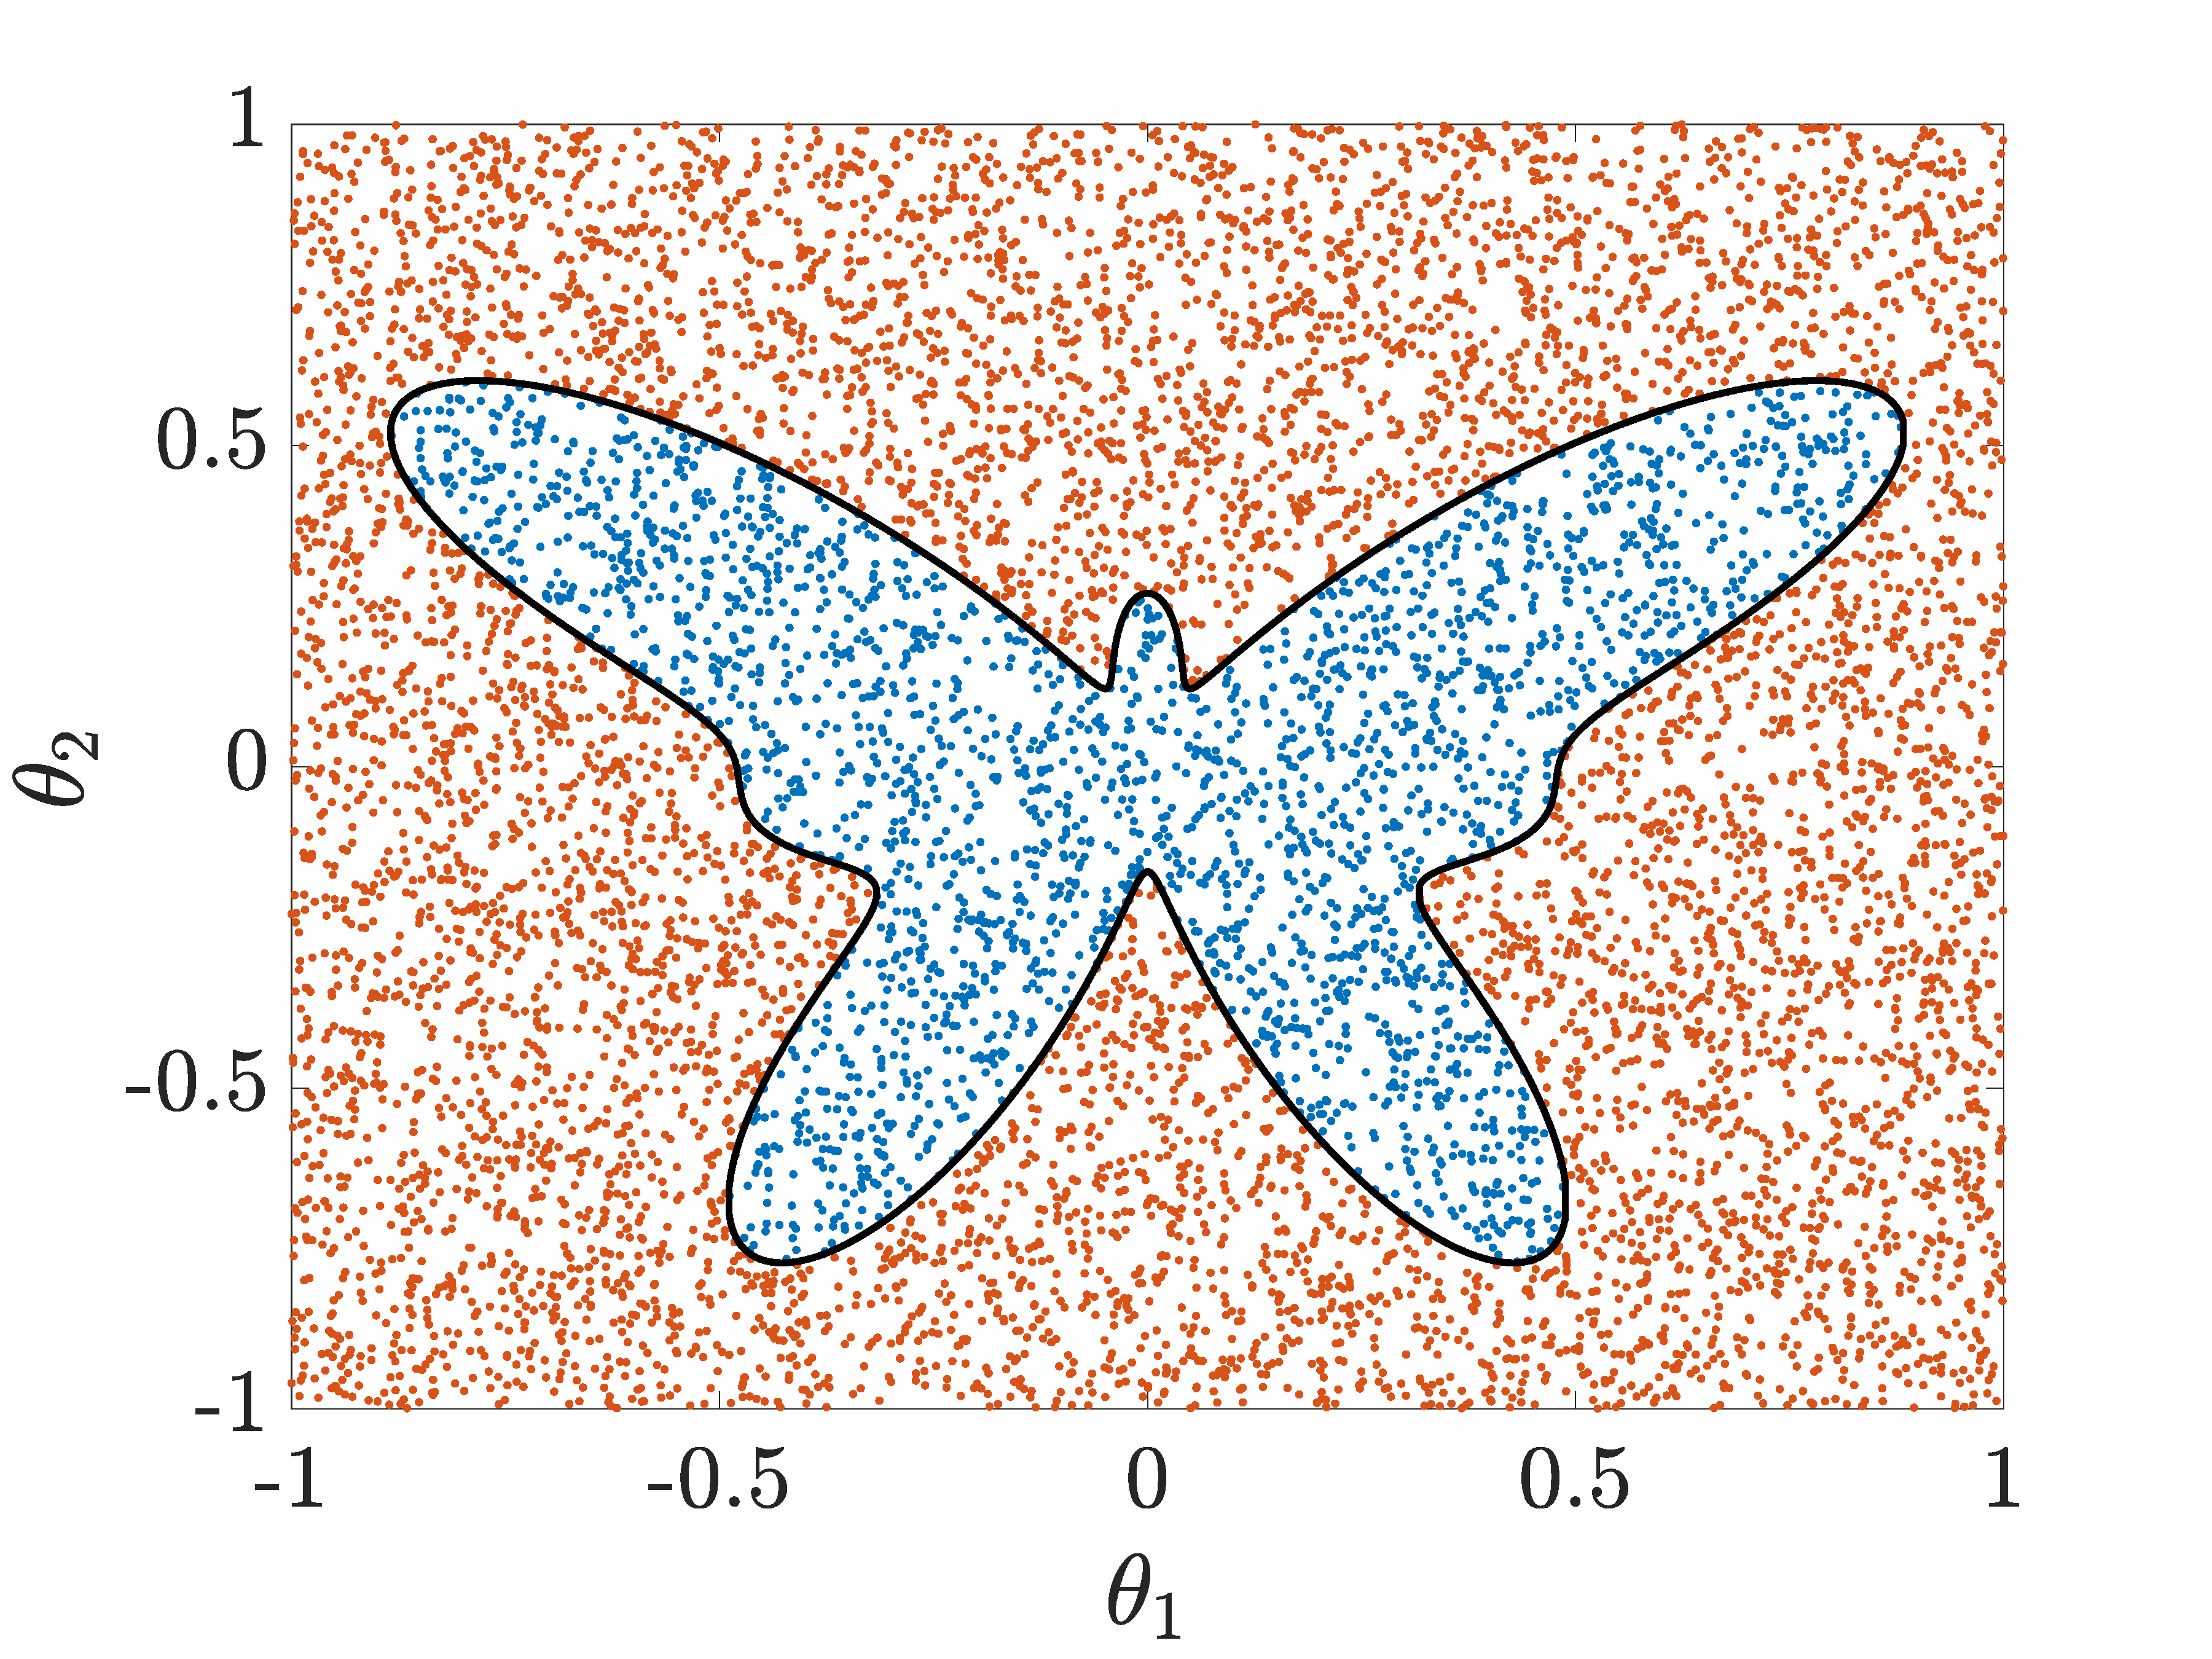
\includegraphics[width=0.6\textwidth]{butterfly}
	\caption{Example of sampling uniformly from an arbitrary shape by 
		rejection.  Here samples are proposed uniformly from the $[-1,1]$
		square.  Any sample falling within the black outline is accepted 
		(blue), otherwise it is rejected (red).  \label{fig:inf:rej-butt}}
\end{figure}

The underlying idea for rejection sampling is that we can sample from any distribution
by sampling uniformly from the hyper-volume under its unnormalized probability density function.
Though this is effectively axiomatic by the definition of a probability density
function with respect to the Lebesgue measure, we can get a non measure-theoretic
intuition for this by considering augmenting a target distribution with a new variable $u$
such that $p(u|\theta) = \textsc{Uniform}(0,\gamma(\theta))$.  Sampling 
$\hat{\theta} \sim \pi(\theta)$ and then $\hat{u}\sim p(u|\theta)$ corresponds to
sampling uniformly from hyper-volume under the probability density function, while we
clearly have that the marginal distribution on $\theta$ is $\pi(\theta)$.

\begin{figure}[t]
	\centering
	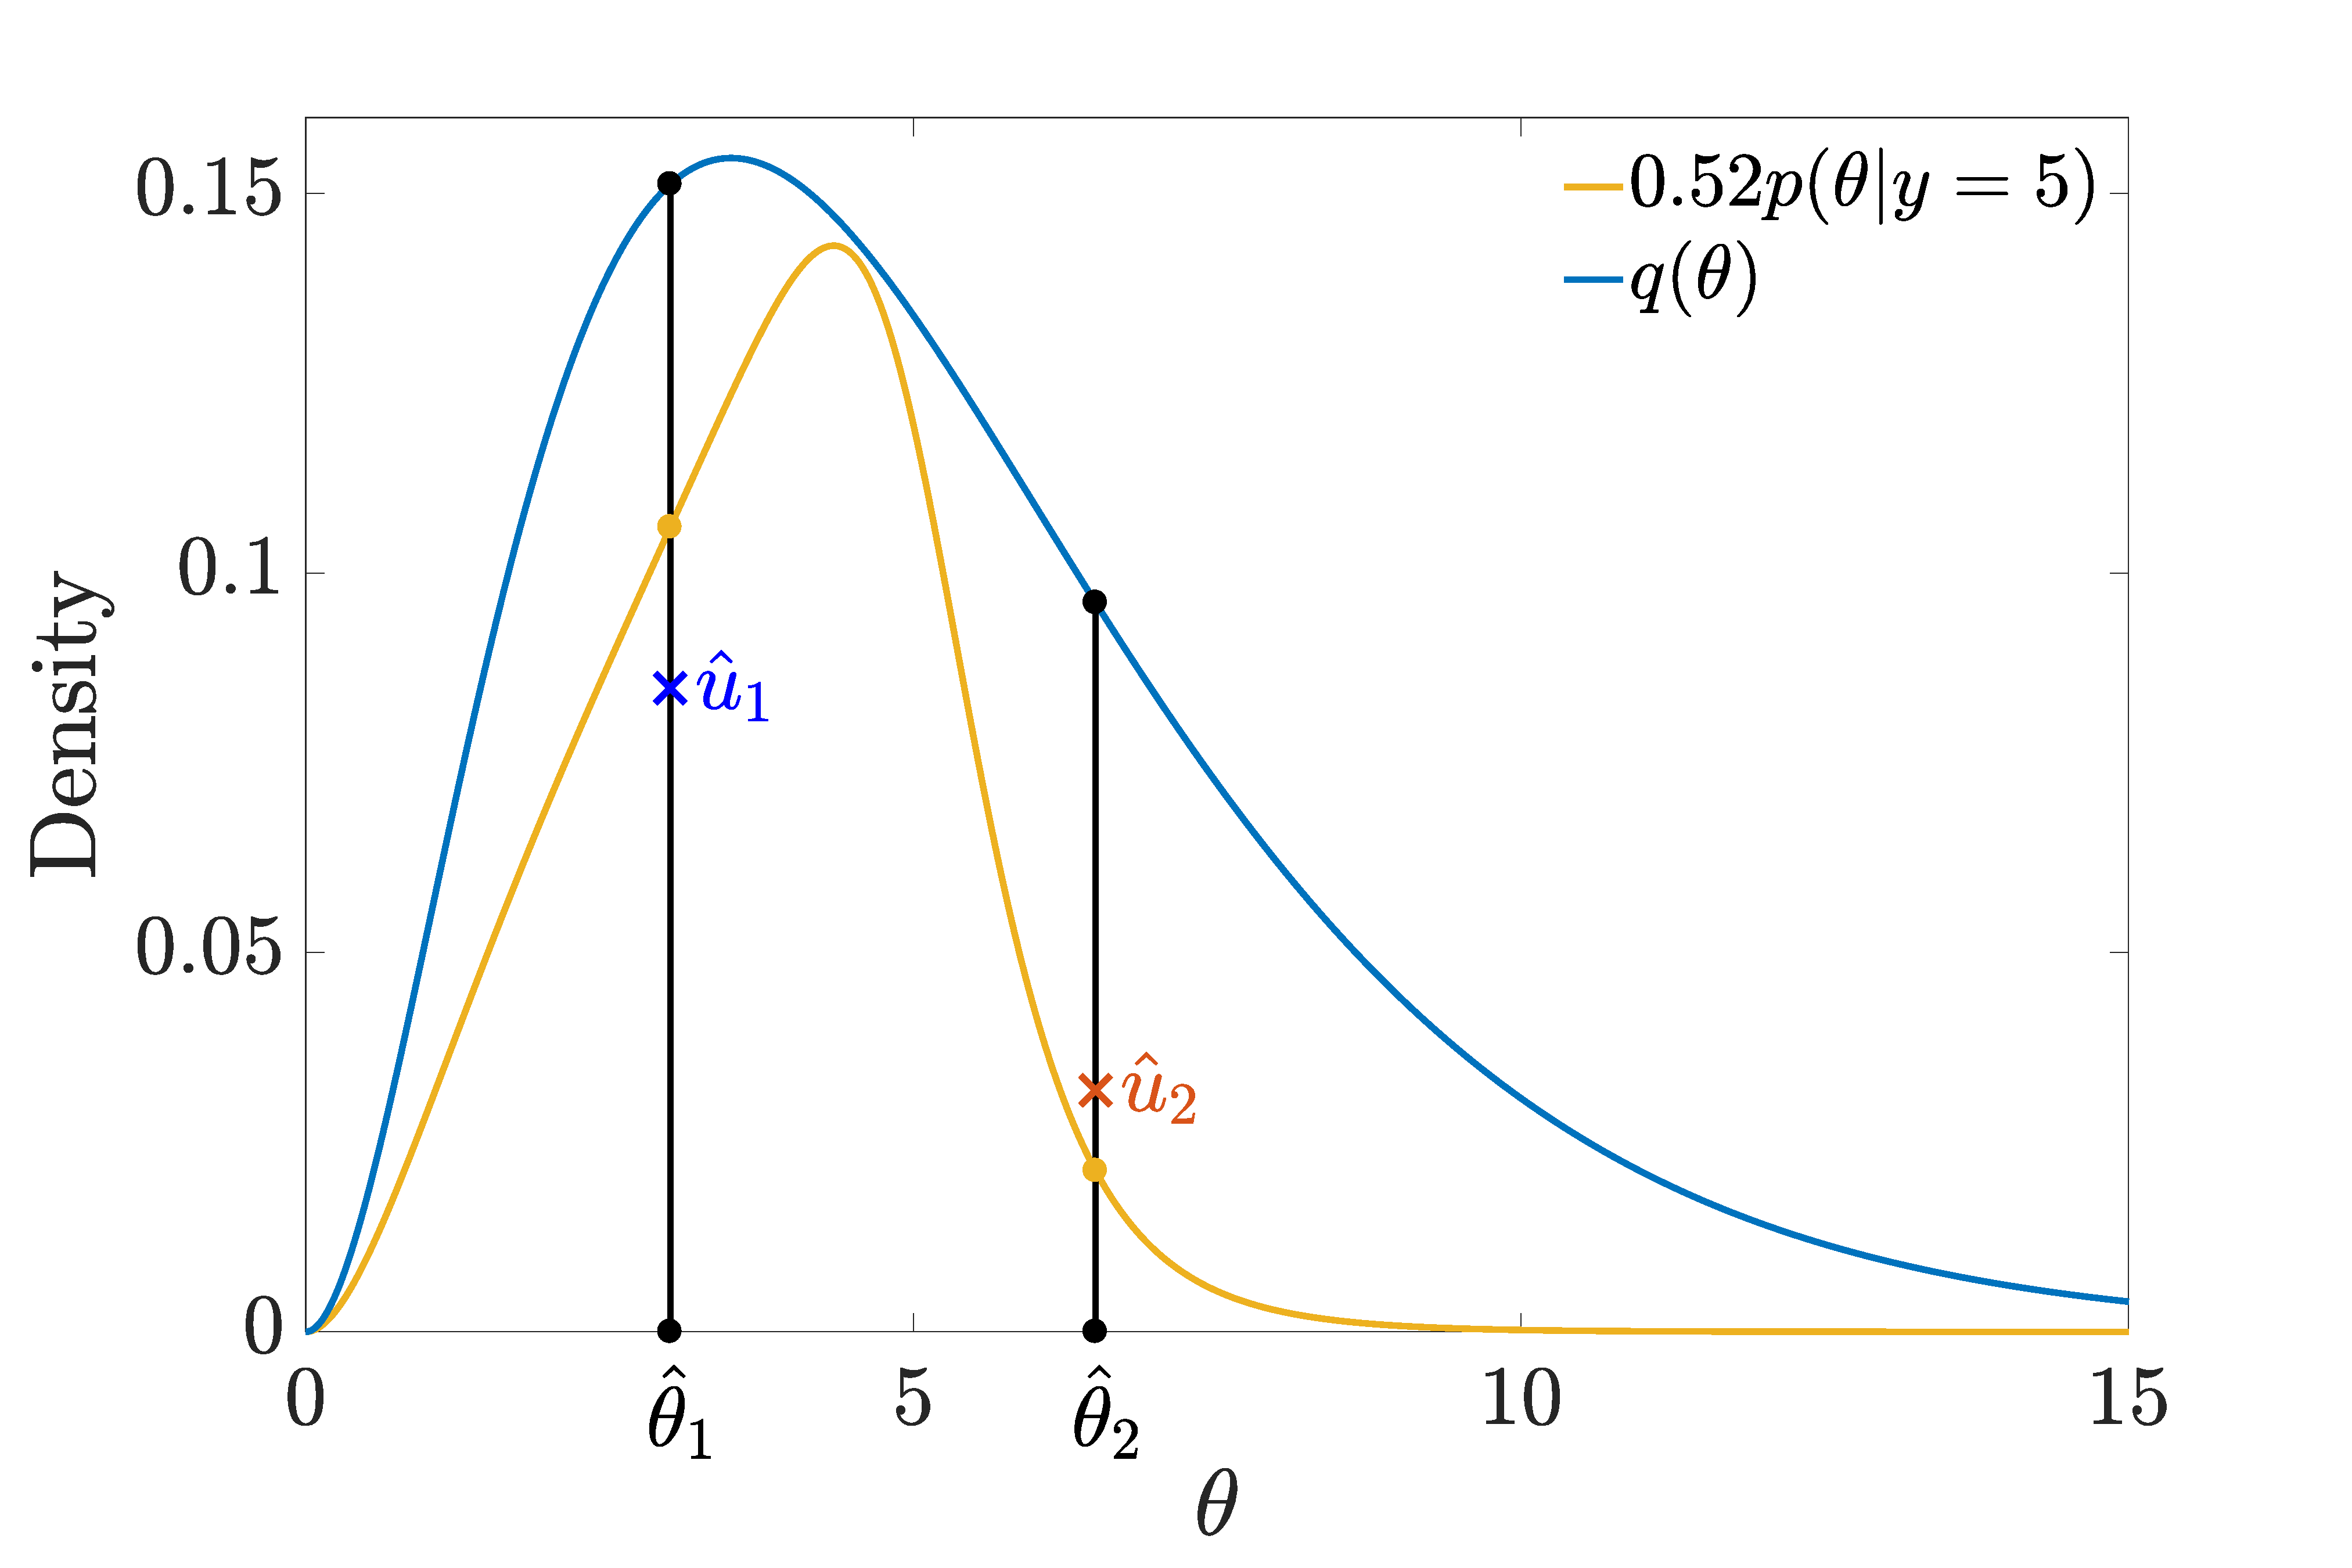
\includegraphics[width=0.7\textwidth]{reject_samp}
	\caption{Demonstration of rejection sampling for problem shown in~\eqref{eq:inf:example}.  
		We first sample $\hat{\theta}\sim q(\theta)$, correspond to the sampling for the distribution
		shown in blue,
		and then sample $\hat{u}\sim \textsc{Uniform}(0,q(\theta))$, corresponding to
		sampling a point uniformly along the black lines for the two shown example values of 
		$\hat{\theta}$.  The point is accepted 
		if $\hat{u} \le C p(\theta | y=5)$ (i.e. if it below the yellow curve) and is 
		otherwise rejected, where we have taken
		$C=0.52$ to ensure $C p(\theta | y=5)\le q(\theta)$ for all theta.
		Here the example sample pair $\{\hat{\theta}_1,\hat{u}_1\}$ is accepted, while
		$\{\hat{\theta}_2,\hat{u}_2\}$ is rejected.  The
		resulting accepted sample pairs will be uniformly sampled from the region under
		the unnormalized target distribution given by the yellow curve and therefore
		the accepted $\hat{\theta}$ will correspond to exact samples from the target.
		 \label{fig:inf:rej-samp}}
\end{figure}

Using this idea, we can sample from any unnormalized distribution by sampling from
an appropriate bounding as per our intuitive example and then accepting only samples
that fall within the hyper-volume of the probability density function. 
More specifically, we define a proposal
distribution $q(\theta)$ which completely envelopes a
scaled version of the unnormalized target distribution $C\gamma(\theta)$ such that 
$q(\theta)\ge C \gamma(\theta)$ for all values of $\theta$ and $C>0$.  We then sample a pair 
$\{\hat{\theta},\hat{u}\}$ by first sampling $\hat{\theta} \sim q(\theta)$ and then
$\hat{u} \sim \textsc{Uniform}(0,q(\theta))$.  The sample is accepted if
\begin{align}
	\label{eq:inf:rej-acc-criteria}
	\hat{u} \le C \gamma(\hat{\theta})
\end{align}
which occurs with an acceptance rate $CZ$ (note that $q(\theta)\ge C \gamma(\theta) \; \forall \theta$
ensures that $C \le 1/Z$).  Note that this can be used to estimate the normalization
constant, corresponding to the marginal likelihood for Bayesian models, by calculating
the empirical estimate of the acceptance rate and dividing this by $C$.
A graphical demonstration of the rejection sampling process is shown in 
Figure~\ref{fig:inf:rej-samp}.

Rejection sampling can be a highly effective sampling or inference method in low dimensions.
In particular, the fact that it generates exact samples from the target distribution can be very
useful.  For example, this characteristic is used to construct efficient samplers for many 
common distributions such as in the ziggurat algorithm~\citep{marsaglia2000ziggurat} often
used for generating Gaussian random variables.  However, its efficiency is critically dependent
on the value of $C$ because it is directly proportional to the acceptance rate.  By proxy, it
is also critically dependent on the proposal $q(\theta)$ as this dictates the minimum possible
value of $C$, namely $C_{\min} = \min_{\theta} q(\theta) Z / \pi(\theta)$.  Note that if 
$q(\theta) = \pi(\theta) \; \forall \theta$ then the acceptance rate will be $1$, while the
more different they are (in terms of $\min_{\theta} q(\theta) / \pi(\theta)$), the lower the
best possible acceptance rate becomes.  In low dimensions, adaptive rejection 
sampling~\citep{gilks1992adaptive} often forms an effective method for adaptively 
learning an effective proposal and corresponding value for $C$, leading to good acceptance
rates.  However, the approach will be very prone to the \emph{curse of dimensionality} as
we discuss in Section~\ref{sec:inf:foundation:curse}, meaning performance cannot be
maintained for higher dimensional problems.
% !TEX root = ../main.tex

\subsection{Importance Sampling}
\label{sec:inf:foundation:importance}

Importance sampling is another common sampling method that forms the key building block
for many more advance inference schemes.  It is closely related to rejection sampling in that
it samples candidate $\hat{\theta}$ from a proposal $q(\theta)$, but instead of going
through an accept/reject step, it assigns an \emph{importance weight} to each sample.
These importance weights act like correction factors to account for the fact that we sampled
from $q(\theta)$ rather than our target $\pi(\theta)$.

To demonstrate the key idea, consider the problem of calculating an expectation as
per~\eqref{eq:inf:expt}.  If we cannot sample exactly from $\pi(\theta)$ then we cannot
apply~\eqref{eq:inf:mc-est} directly.  However, we can rearrange the form our expectation
to generate a different \mc estimator which we can evaluate directly as follows
\begin{align}
	I:=\E_{\pi(\theta)} \left[f(\theta)\right] &=\int f(\theta) \pi(\theta) d\theta 
	= \int f(\theta) \frac{\pi(\theta)}{q(\theta)} q(\theta) d\theta \nonumber \\
	&\approx \frac{1}{N} \sum_{n=1}^{N} \frac{\pi(\hth_n)}{q(\hth_n)} f(\hat{\theta}_n)
	\quad \text{where} \quad \hat{\theta}_n \sim q(\theta) 	\label{eq:inf:importance}
\end{align}
where $\frac{\pi(\hth_n)}{q(\hth_n)} =: w_n$ is known as an importance weight.
The key trick we have applied is to multiply the integrand by $\frac{q(\theta)}{q(\theta)}$, which
equals $1$
for all points where $q(\theta) \neq 0$.  Thus if $q(\theta) \neq 0$ for all $\theta$ for which
$\pi(\theta) \neq 0$ (to avoid infinite importance weights), this has no effect on the 
expectation.  However, we can informally view the new
formulation as being the expectation of $f(\theta) \frac{\pi(\theta)}{q(\theta)}$ under the
distribution $q(\theta)$.  We can now construct a \mc estimator for this new formulation, 
by choosing $q(\theta)$ to be a distribution we can sample from.  A graphical
demonstration of importance sampling is given in Figure~\ref{fig:inf:importance} in the
more general setting where we do not have access to the $\pi(\theta)$ exactly, but only
an unnormalized version $\gamma(\theta)=\pi(\theta)Z$.  As we will show in detail in
Section~\ref{sec:inf:foundation:importance:self-norm}, we can still use importance sampling
in this case by \emph{self-normalizing} the weights.

\begin{figure}[t]
	\centering
	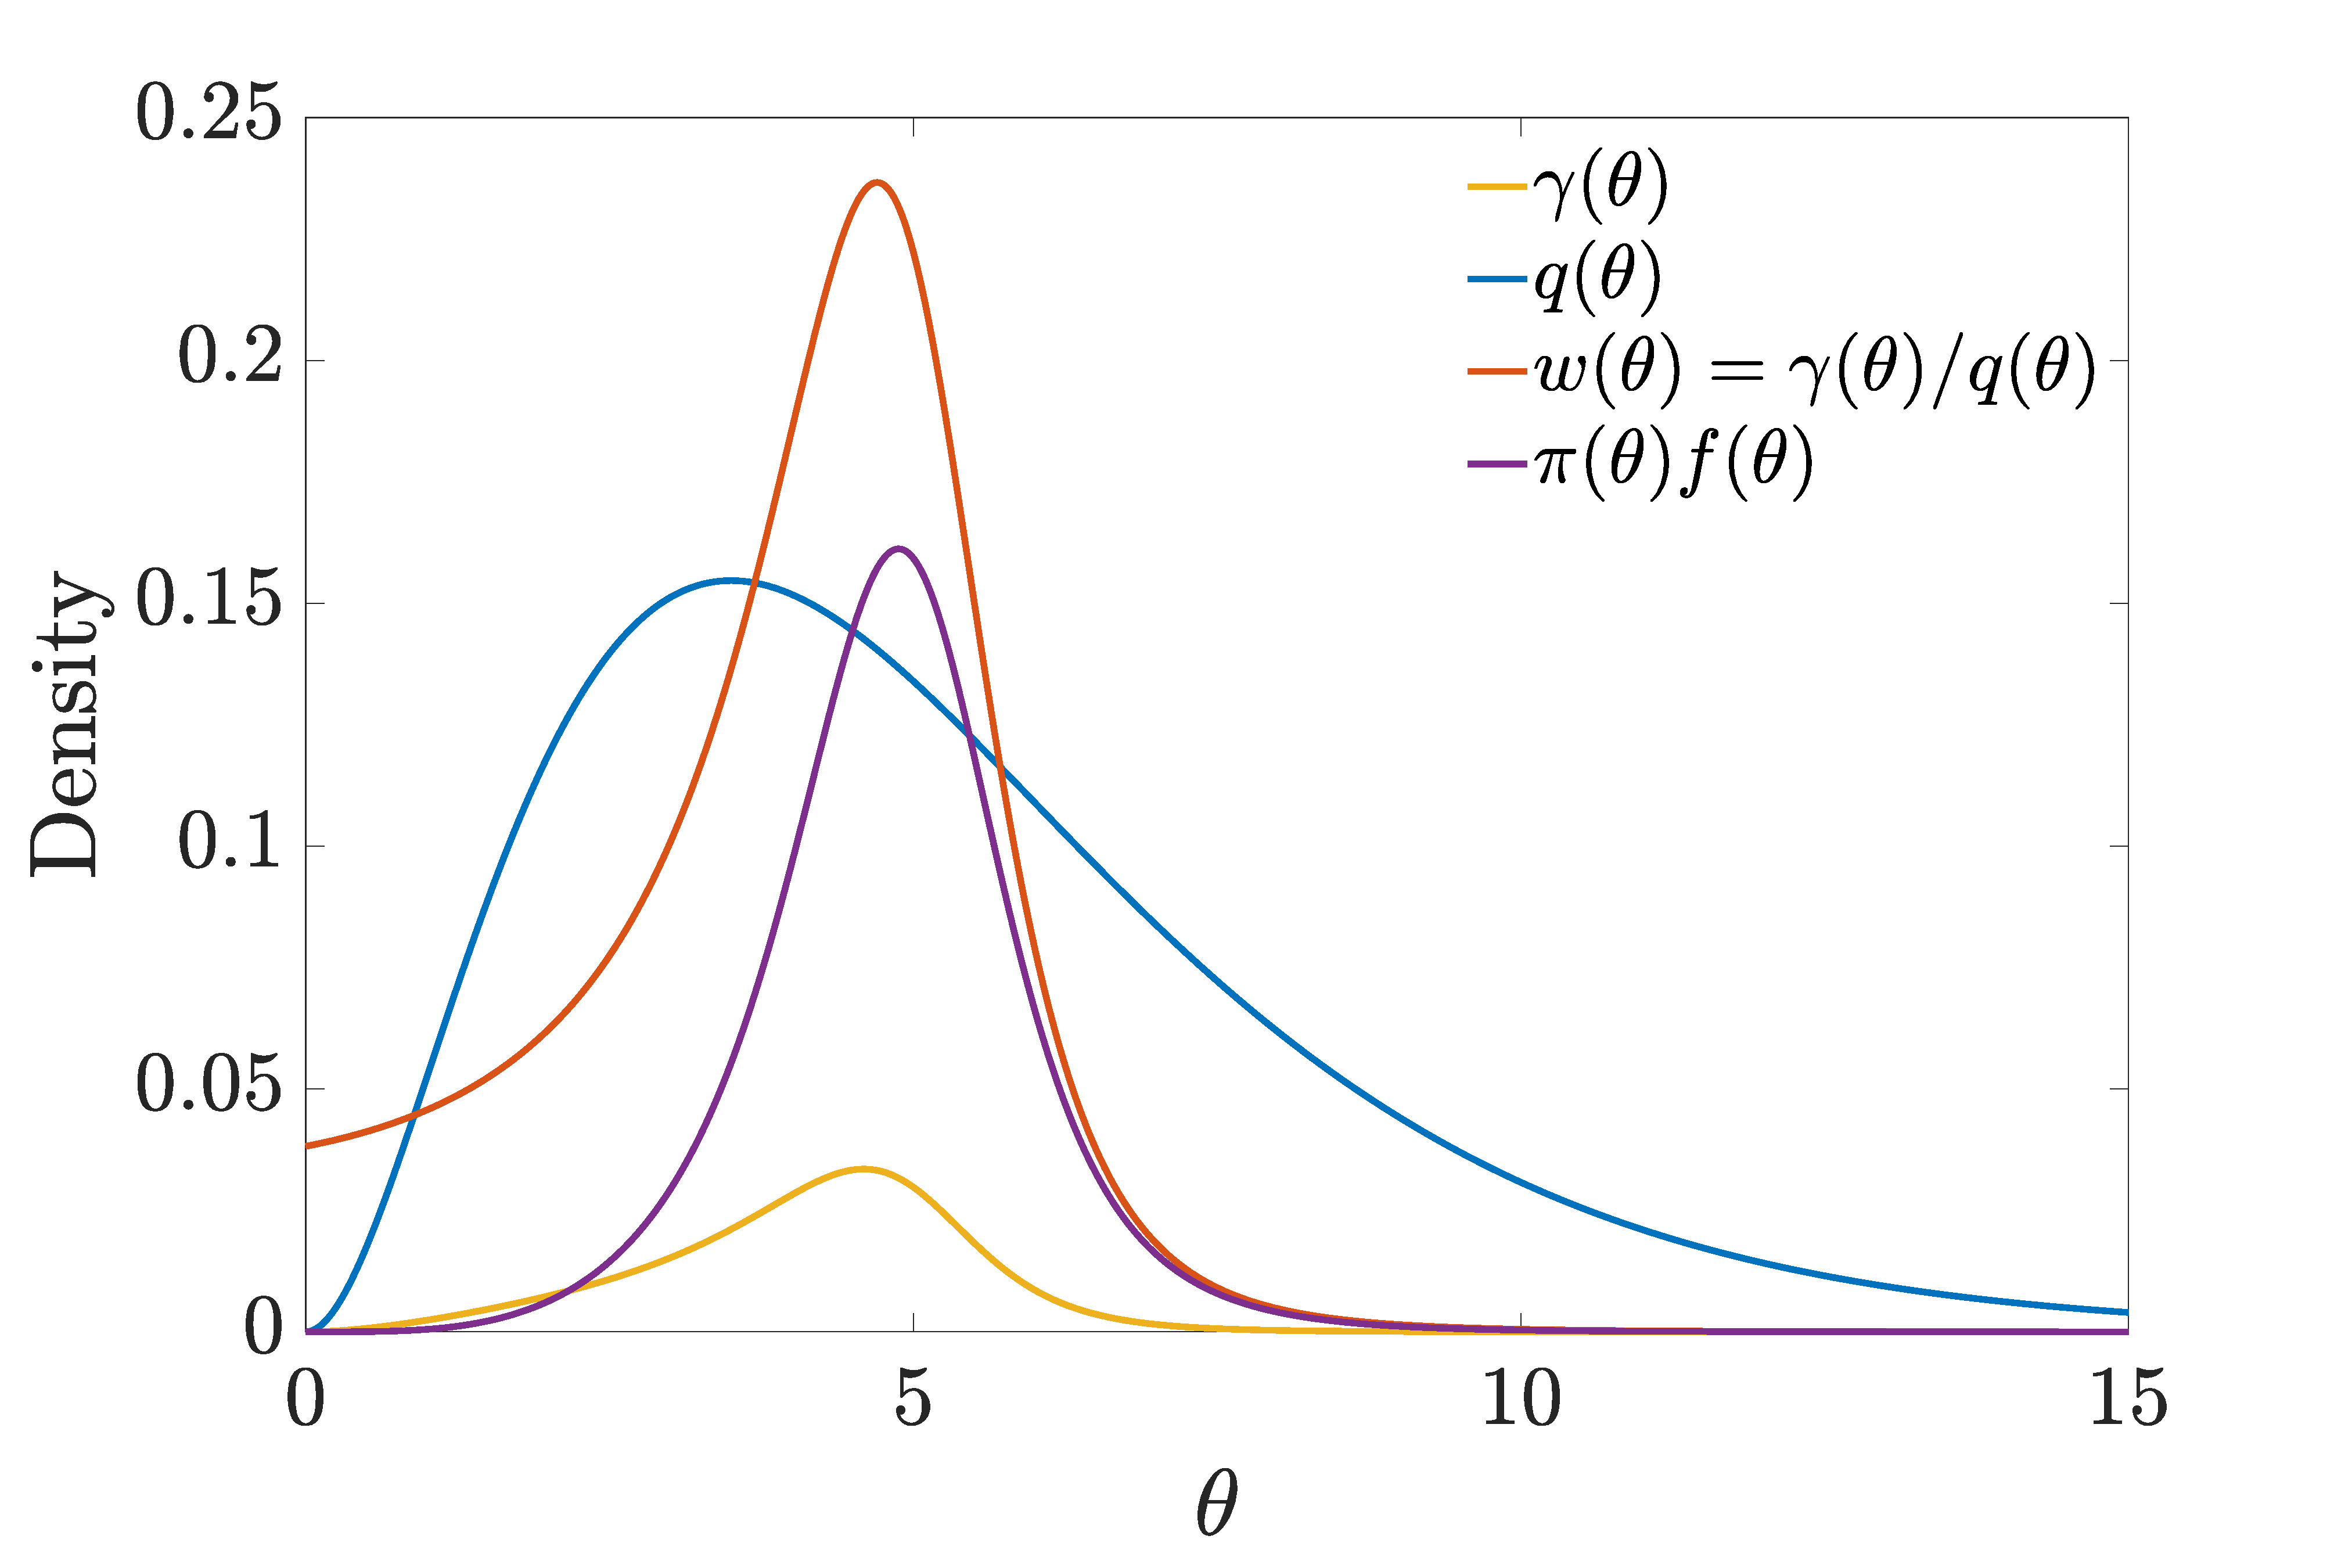
\includegraphics[width=0.7\textwidth]{importance}
	\caption{Demonstration of importance sampling for problem shown in~\eqref{eq:inf:example}
		where we are trying to estimate $\E [\pi(\theta)f(\theta)]$: the expectation of the function $f(\theta) := \theta^2/50$
		under the posterior $\pi(\theta):=p(\theta|y=5)$ defined as per~\eqref{eq:inf:example-post}.
		We assume the setting where $\pi(\theta)$ is only known up to a normalization constant
		(see Section~\ref{sec:inf:foundation:importance:self-norm}), namely we only have access
		to $\gamma(\theta) := p(\theta)p(y=5 | \theta)$ as shown in yellow.  Our procedure is to draw
		samples independently $\hth_n \sim q(\theta)$ and then evaluate their weight 
		$w_n = w(\hth_n) = \gamma(\hth_n)/q(\hth_n)$.  This produces a set of weighted samples
		which can then be used to estimate to estimate the expectation using~\eqref{eq:inf:snis}
		(one can also use~\eqref{eq:inf:importance} if the normalized $\pi(\theta)$ is used instead of
		$\gamma(\theta)$).
		\label{fig:inf:importance}}
\end{figure}

Importance sampling has a number of desirable properties as an inference method.
In particular, it is both unbiased and consistent.  The former can be shown trivially
as follows
\begin{align}
\E \left[\frac{1}{N} \sum_{n=1}^{N} \frac{\pi(\hth_n)}{q(\hth_n)} f(\hat{\theta}_n)\right] &=
\frac{1}{N} \sum_{n=1}^{N} \E _{q(\theta_n)}\left[\frac{\pi(\hth_n)}{q(\hth_n)} f(\hat{\theta}_n)\right] \nonumber \\
&=\E _{q(\theta_1)}\left[\frac{\pi(\hth_1)}{q(\hth_1)} f(\hat{\theta}_n)\right] =
\E _{\pi(\theta)}\left[f(\theta)\right]
\end{align}
where we have effectively stepped backwards through~\eqref{eq:inf:importance}.
Given this unbiasedness result, $L^2$ convergence, and thus convergence in probability,
can be shown in the same manner as~\eqref{eq:inf:LLN-informal} by replacing
each $f(\hth_n)$ with $\frac{\pi(\hth_n)}{q(\hth_n)} f(\hat{\theta}_n)$, leading to the
same result except that $\sigma_{\theta}$ is now
\begin{align}
\label{eq:inf:sigma-imp}
\sigma_{\theta}^2 = \E_{q(\theta)} \left[\left(\frac{\pi(\hth_n)}{q(\hth_n)} f(\hat{\theta}_n)-I\right)^2\right]
= \var_{q(\theta)} \left[\frac{\pi(\theta)}{q(\theta)} f(\theta)\right].
\end{align}
Almost sure convergence of importance sampling can be similarly shown using
the strong law of large numbers.

The form of~\eqref{eq:inf:sigma-imp} provides substantial insight into how
best to set the proposal: we have shown that the mean squared error of an
importance sampler is directly proportional to $\var \left[f(\theta)\pi(\theta)/q(\theta)\right]$,
thus the lower this term is, the better the expected performance of our
estimator.  One obvious question is what is the optimal proposal $q^*(\theta)$?
It turns out that $q^*(\theta) = \frac{\pi(\theta)\left|f(\theta)\right|}
{\int \pi(\theta)\left|f(\theta)\right|d\theta}$
\citep{kahn1953methods,owen2013mc}, which can be
 shown as follows where we will make use of Jensen's inequality
\begin{align}
\var_{q^*(\theta)} &\left[\frac{\pi(\theta)}{q^*(\theta)} f(\theta)\right] =
\E_{q^*(\theta)} \left[\left(\frac{\pi(\theta)}{q^*(\theta)} f(\theta)\right)^2\right]
-\left(\E_{q^*(\theta)} \left[\frac{\pi(\theta)}{q^*(\theta)} f(\theta)\right]\right)^2
\nonumber \\
 &= \int \frac{\pi(\theta)^2 f(\theta)^2}{q^*(\theta)} d\theta
 -I^2 
 = \left(\int \pi(\theta) \left|f(\theta)\right| d\theta\right)^2
 -I^2 \label{eq:inf:opt-q-line2}\\
 &\le \int \left(\frac{\pi(\theta) f(\theta)}{q(\theta)}\right)^2 q(\theta) d\theta
 -I^2 =\var_{q(\theta)} \left[\frac{\pi(\theta)}{q(\theta)} f(\theta)\right] \label{eq:inf:opt-q}.
\end{align}
Here we have shown that the variance for $q^*(\theta)$ is less than or equal to the variance
using an arbitrary $q(\theta)$.  It must therefore be the optimal proposal.
A further point of note is that if $f(\theta)\ge0 \; \forall \theta$ (or 
$f(\theta)\le0 \; \forall \theta$), 
then~\eqref{eq:inf:opt-q-line2} will equal zero giving a zero variance estimator:
each importance weight will be equal to the  $I/f(\theta)$ and thus $I$
can be calculated by evaluating a single point.  

Though it will typically be impossible to find $q^*(\theta)$ in practice, it still 
provides a guide as to what constitutes a good proposal -- we want
$\pi(\theta)\left|f(\theta)\right|/q(\theta)$ to be a close to constant as possible.
In particular, we need to be careful to avoid scenarios where 
$\frac{\pi(\theta)\left|f(\theta)\right|}{\int \pi(\theta)\left|f(\theta)\right|d\theta}
\gg q(\theta)$ as this will cause the ratio to explode, leading to high variances.
A consequence of this is that we want $q(\theta)$ to have \emph{light tails}
compared to $\pi(\theta)\left|f(\theta)\right|$ to ensure that the ratio does not
systematically increase as $\theta$ moves away from the modes of $q(\theta)$.
Aside from the clear practical issues, If this requirement does not hold, then
it can easily be the case that $\sigma_{\theta}=\infty$ and thus that the estimator
has infinite variance.  Consider, for example, the case where 
$\pi(\theta) = \mathcal{N}(\theta ; 0,1)$, $f(\theta)=\theta$, and
$q(\theta) = \mathcal{N}(\theta ; 0,s^2)$ (Example 9.1 from~\cite{owen2013mc}).
Noting that the mean, $I$, is zero by symmetry and defining $\nu = \frac{1}{2s^2}-1$, we have that
%, $\mathrm{erf}$ is the error function for which $\mathrm{erf}(\infty)=-\mathrm{erf}(-\infty)=1$)
\begin{align}
\sigma_{\theta}^2 &= \int_{-\infty}^{\infty} \theta^2 \frac{\left(\exp\left(-\theta^2/2\right)/\sqrt{2\pi}\right)^2}
{\exp\left(-\theta^2/\left(2s^2\right)\right)/\sqrt{2\pi s^2}} d\theta
-I^2 \nonumber \\
&= \frac{s}{\sqrt{2\pi}}  \int_{-\infty}^{\infty} \theta^2 \exp \left(\theta^2 \nu\right) d\theta.
%&= \frac{s}{\sqrt{2\pi}}  \int_{-\infty}^{\infty} \theta^2 \exp \left(-\frac{\theta^2}{2}\left(2-\frac{1}{s^2}\right)\right) d\theta
%&= \frac{s}{\sqrt{2\pi}}  \left[
%\frac{\sqrt{\frac{\pi}{2}} \mathrm{erf} \left(\frac{\theta}{\sqrt{2}} \sqrt{2-\frac{1}{s^2}}\right)}
%{\left(2-\frac{1}{s^2}\right)^{3/2}}-\frac{\theta \exp \left(-\frac{\theta^2}{2}\left(2-\frac{1}{s^2}\right)\right) }{\left(2-\frac{1}{s^2}\right)}
%\right]_{\theta=-\infty}^{\theta=\infty} \nonumber \\
%&= \frac{s}{\left(2-\frac{1}{s^2}\right)^{3/2}}
\end{align}
Now this integral is clearly only finite for $\nu < 0$ (as otherwise the integrand
is $+\infty$ and $\theta = \pm \infty$ and finite elsewhere).  Therefore, $\sigma_{\theta}$
is only finite when $s^2>1/2$.  In other words, we only get a finite estimator
in this case if the proposal variance is at least half that of the target distribution $\pi(\theta)$.
The highlights the pitfalls of having insufficiently heavy tails on our proposal.
Overcoming these will typically require careful setup of the proposal on a case-by-case basis,
for example, choosing a distribution type for the proposal that is known to have heavier tails 
than $\pi(\theta)$.

\subsubsection{Self-Normalized Importance Sampling}
\label{sec:inf:foundation:importance:self-norm}

In the previous section we presumed that we have access to a normalize version of the target
$\pi(\theta)$.  Typically this will not be the case and we will only have access to an
unnormalized target $\gamma(\theta)=\pi(\theta)Z$ as per~\eqref{eq:inf:unnorm-target},
for example only having access to the joint rather than the posterior in the Bayesian inference setting.
In a less common but still plausible situation, it may also only be possible to evaluate the proposal
up to a normalization constant.
We now show how one can still use importance sampling in these scenarios, by
\emph{self-normalizing} the importance weights.

The key idea for self-normalized importance sampling (SNIS) is that the weights provide
an unbiased and consistent estimator of the marginal likelihood
\begin{align}
Z_N &= \frac{1}{N} \sum_{n=1}^{N} w_n, \\
\E [Z_N] &= \frac{1}{N} \sum_{n=1}^{N} \E[w_n] =\E_{q(\hth_1)}[\gamma(\hth_1)/q(\hth_1)] = Z.
\end{align}
Now as $\E_{q(\theta)}\left[\frac{\gamma(\theta)}{q(\theta)}f(\theta)\right]=
E_{q(\theta)}\left[\frac{\pi(\theta)}{q(\theta)} Zf(\theta)\right]=Z\;\E_{\pi(\theta)} \left[f(\theta)\right]$, we can 
use our samples to construct \mc estimators for both $Z$ and $Z\;\E_{\pi(\theta)} \left[f(\theta)\right]$ and use the ratio
of our estimates to get an estimate for $E_{\pi(\theta)} \left[f(\theta)\right]$
\begin{align}
\label{eq:inf:snis}
\E_{\pi(\theta)} \left[f(\theta)\right] \approx \frac{\sum_{n=1}^{N} w_n f(\hth_n)}{\sum_{n=1}^{N} w_n}
\quad \mathrm{where} \quad \hth_n \sim q(\theta), \quad w_n = \frac{\gamma(\hth_n)}{q(\hth_n)}.
\end{align} 
This can alternatively be expressed as
$\E_{\pi(\theta)} \left[f(\theta)\right] \approx \sum_{n=1}^{N} \bar{w}_n f(\hth_n)$
where $\bar{w}_n = \frac{w_n}{\sum_{n} w_n}$ are the normalized importance 
weights such that $\sum_{n=1}^N\bar{w}_n = 1$.  

The consistency of~\eqref{eq:inf:snis} follows
directly from the individual consistency of both the numerator and the denominator to 
$Z\;\E_{\pi(\theta)} \left[f(\theta)\right]$ and $Z$ respectively.
However, unlike~\eqref{eq:inf:importance},~\eqref{eq:inf:snis} is biased estimator
for finite $N$.  This is
because the numerator and denominator are correlated and because 
even though $Z_N$ is an unbiased estimator of $Z$, $1/Z_N$ is not an unbiased
estimator of $1/Z$. The latter follows directly from Jensen's inequality
noting that inversion is a convex function for strictly positive inputs,
\begin{align}
\E \left[\frac{1}{\sum_{n=1}^{N} w_n}\right] \ge \frac{1}{\E \left[\sum_{n=1}^{N} w_n\right]} = \frac{1}{Z},
\end{align}
where equality holds only if $Z_N$ is a zero variance estimator for $Z$ (which
typically happens only in the limit $N\rightarrow\infty$).  However, it can be shown that the
bias decreases at a rate $O(1/N)$ (see e.g.~\cite{doucet2009tutorial}), whereas the
standard deviation of the estimate decreases at a rate $O(1/\sqrt{N})$.  Thus the bias
becomes dominated as $N\rightarrow\infty$.
Strangely, even when the normalization constant
is known, the self-normalized importance sampler can still be lower variance~\citep{owen2013mc}.
Therefore, with the bias becoming dominated, it can actually be preferable to use
SNIS even when the normalized target is known.  Note also that the optimal proposal in
the SNIS case varies slightly from the $q^*(\theta)$ derived earlier in the Section
and is instead~\citep{hesterberg1988advances}
\begin{align}
q^*_{\mathrm{SNIS}} (\theta) = \frac{\pi(\theta)\left|f(\theta)-I\right|}
{\int \pi(\theta)\left|f(\theta)-I\right|d\theta}.
\end{align}
As a consequence, there is a minimum variance on the SNIS estimator, unlike in the
pre-normalized case where $q^*(\theta)$ was a zero variance estimator  was possible
if $f(\theta)\ge0 \; \forall \theta$.

\subsubsection{Unknown $f$}
\label{sec:inf:foundation:importance:unk-f}

So far we have assumed that we are using importance sampling to calculate an expectation 
of a known function.  In practice, there will be many scenarios, particularly in the Bayesian inference setting,
where $f(\theta)$ is not known ahead of time and we instead desire to generate samples
for some future unknown use.  For example, in Section INSERT we will introduce the concept
of \emph{sequential Monte Carlo} where we will typically have multiple importance sampling steps
before any target function is itself evaluated.
When no $f(\theta)$ is specified we can carry out importance sampling in the
same fashion, sampling from $q (\theta)$ and returning a set of \emph{weighted} samples
$\{\hth_n,w_n\}_{n=1:N}$ where the weights are equal to $\gamma(\hth_n) / q(\hth_n)$ as before.
Here we can think of importance sampling as approximating the posterior with a series of deltas
functions, namely
\begin{align}
\label{eq:inf:imp-post-est}
\pi (\theta) \approx \hat{\pi}(\theta) := \sum_{n=1}^{N} \bar{w}_n \delta_{\hth_n} (\theta)
\end{align}
where $\delta_{\hth_n} (\theta)$ are delta functions centred at $\hth_n$.

Importance weights are multiplicative when doing conditional
sampling: if we sample $\hth_n \sim q_1(\theta)$ then $\hat{\phi}_n | \hth_n \sim q_2(\phi | \hth_n)$
when targeting $\gamma_1(\theta)\gamma_2(\phi|\theta)$ then the importance weight is 
\begin{align}
\label{eq:inf:prod-imp-weights}
\frac{\gamma_1(\hth_n)\gamma_2(\hat{\phi}_n|\hth_n)}{q_1(\hth_n)q_2(\hat{\phi}_n | \hth_n)}
=\frac{\gamma_1(\hth_n)}{q_1(\hth_n)}
\times\frac{\gamma_2(\hat{\phi}_n|\hth_n)} {q_2(\hat{\phi}_n | \hth_n)}= w_{n,1} \times w_{n,2}.
\end{align}
This is known as sequential importance sampling and means that we can propagate importance
weighted samples through a computational system and retain a valid importance
sampler with the standard properties such as unbiasedness (presume the weights are not self-normalized) 
and consistency.\footnote{Note that
	this does not apply to the \emph{nested estimation} case as we discuss in
	Chapter~\ref{chp:nest}.} 

Again a natural question in this ``unknown $f$'' setting is what is the optimal proposal $q^*(\theta)$?
This is a somewhat more challenging and subjective question than when $f$ is known as the
optimality will depend on what the samples are eventually used for.  In particular, even if we do
not known $f$ precisely, it may be the case that we believe some $f$ are more likely than others or we
may know that $f$ lives within some space of possible functions, for example functions that have
a countable number of discontinuities.  

One simple, but insightful approach, is to consider the 
\emph{minimax} optimal proposal, i.e. the proposal that has the minimum error if $f$ is the
most adversarial possible function for that proposal.
Imagine that we have $N$ weighted samples
$\{\hth_n,w_n\}_{n=1:N}$, with $N$ corresponding evaluations $f_n := f(\hth_n)$.
We use these to calculate an estimate $I_N$ for the target $I$.
Now assume that each $w_n\ge0$, $\sum_{n=1}^{N}w_n = 1$, and $\sum_{n=1}^{N} |f_n-I| = N$ to
preclude the ability to provide an improved solution simply by scaling the problem.
The error for the estimator is given by
\begin{align}
\left|I_N-I\right| = \left|\sum_{n=1}^{N} w_n f_n - I\right| = \left|\sum_{n=1}^{N} w_n (f_n - I)\right|.
\end{align}
For any given set of weights, the most adversarial set of function evaluations is
to have all our error at the largest weight, i.e. $|f_{n^*}-I| = N$ and $|f_{n}-I| = 0, \; n\neq n^*$
where $n^*$ is the index of the largest weight.  For this set of adversarial $f_n$, the
lowest error is achieved when each of the weights are equal.  Consequently,
we see that the minimax proposal under our assumptions is $q(\theta)=\pi(\theta)$.
This result is perhaps not surprising as it effectively states that the best sample representation 
of $\pi(\theta)$ for an unknown future use is to sample from that distribution directly.
As shown in the next section, this proposal will also minimize the variance of the estimator
under the assumption that the $f_n$ are independent.

Nonetheless, this point of view is not without criticism in the 
literature~\citep{o1987monte,ghahramani2003bayesian,briol2015probabilistic}.  Most of 
this criticism revolves around the valid point that in practice the value of $f(\theta)$ 
does convey information about $f(\theta+\varepsilon)$ and so the correlation between 
samples such be taken into account when making an estimation.  Though the thrust of
this argument is mostly directed towards changing the Monte Carlo method, and in particular
importance sampling, at a more fundamental level, the same arguments would still suggest
that it is can be beneficial to use a proposal that is more diffuse than the target, thereby
reducing the correlation between the produced samples.

\subsubsection{Effective Sample Size}
\label{sec:inf:foundation:ess}

In this section we consider an important diagnostic for the performance of importance
sampling based schemes, the \emph{effective sample size} (ESS).  In
Section~\ref{sec:inf:mc:clt} we showed how an uncertainty estimate for a \mc
estimator can be derived.  However, this does cannot be used when $f$ is unknown
and even if $f$ is known, it does necessarily convey much information about how effective
our proposal is compared to how effective it could be.  The ESS instead informally provides an
estimated measure of the amount of information stored in our weighted sample set.
The more information stored in the samples, the better our approximation of the posterior, and,
at a high level, the more evenly balanced our weights, the more information they encode.
Therefore, the ESS is a measure of how many unweighted samples would be required to
convey the same information about the posterior as the weighted sample set.

The weighted average of $N_e$ independent evaluations $\{f_n\}_{n=1}^N$, each 
with individual variance $\sigma^2$,
has variance $\sigma^2 / N_e$ as we showed in~\eqref{eq:inf:LLN-informal}.  Therefore,
we can calculate the ESS of a set of weighted samples by comparing the variance of our 
weighted estimated to the variance of an estimate using a
set of unweighted evaluations  More specifically, the ESS will be the number of unweighted evaluations
$N_e$ that gives an equivalent variance to our weighted estimate as follows where we
will make use of the assumption that the $f_n$ are independent
\begin{align}
\frac{\sigma^2}{N_e} &= \var \left[\frac{\sum_{n=1}^{N} w_n f_n}{\sum_{n=1}^{N} w_n} \middle| 
														\{w_n\}_{n=1}^N\right] \nonumber \\
&= \sum_{n=1}^{N} \left(\frac{\sum_{n=1}^{N} w_n}{\sum_{n=1}^{N} w_n} \right)^2 \var [f_n] \nonumber \\
&= \frac{\sigma^2\sum_{n=1}^{N} w_n^2}{\left(\sum_{n=1}^{N} w_n\right)^2}.
\end{align}
Now rearranging for $N_e$ we get
\begin{align}
\label{eq:inf:ess}
N_e = \frac{\left(\sum_{n=1}^{N} w_n\right)^2}{\sum_{n=1}^{N} w_n^2} = \frac{1}{\sum_{n=1}^{N} \bar{w}_n^2}
\end{align}
which completes our definition for the effective sample size other than in some scenarios
it is necessary to collapse identical weighted samples to a single sample when
calculating~\eqref{eq:inf:ess}, such as when doing doing resampling (see Section~\ref{sec:inf:foundation:resampling}).  
It transpires that $N_e$ is
independent of $f$, so we can still use the ESS as a diagnostic when $f$ is unknown.
It is straightforward to show using Jensen's inequality we have that $N_e\le N$ with equality
holding if and only if all the weights are equal.  On the other hand, if all but one of the weights
is zero, then $N_e=1$.  These two extremes respectively occur when the proposal
is equal to the target, $q(\theta)=\pi(\theta)$, and when the proposal provides a very poor
representation of the target.  The ESS is often therefore used for \emph{proposal adaptation},
as a larger value of the ESS generally indicates a better proposal.

However, the ESS is far from a perfect measure of sample quality.  For example, if the proposal
perfectly matches one of the modes of the target but completely misses another larger mode, the
ESS will usually be very high, even though the samples provide a very poor representation of the
target.  It is not uncommon in practice to see the ESS drop drastically as more samples are added,
due to the addition of a new dominating sample, typically indicating a region of significant target probability
mass that had previously been missed.  Nonetheless, the ESS is still a very useful performance
metric and is usually a reliable indicator for whether our importance sampling is struggling.  
In particular, though the possibility of missing modes means that it is possible for the ESS to be 
high even when the approximation of the posterior is poor, if the ESS is low then the approximation 
of the posterior will always be poor and any subsequent estimates will, in general, be high variance.

\subsubsection{Resampling}
\label{sec:inf:foundation:resampling}

A useful feature of SNIS is that it can be used to produce unweighted samples
by \emph{sampling with replacement} from the set of produced samples in proportion
to the sample weights.  This procedure is typically known as resampling, because we
are resampling samples from the empirical distribution of our original samples.
It allows us to generate unweighted samples with importance sampling which are
approximately distributed according to $\pi(\theta)$, with this approximation becoming
exact in the limit $N\rightarrow\infty$.  
Resampling on its own always lead to a higher variance estimator than using~\eqref{eq:inf:snis}
directly.   However, in addition to  being necessary when unweighted samples are required,
it will be a key component in the so-called particle-based inference methods discussed
in Chapter INSERT.  For example, when interleaved with sequential importance sampling,
this leads to the sequential importance resampling algorithm which is the backbone of 
sequential \mc methods.

Mathematically, we can express resampling as producing a set unweighted resampled
samples $\left\{\tilde{\theta}_n\right\}_{n=1}^N$ using
\begin{align}
\label{eq:inf:resampling}
\tilde{\theta}_n = \hth_{a_n} \quad \mathrm{where} \quad
a_n \sim \textsc{Discrete}\left(\left\{\bar{w}_n\right\}_{n=1}^N\right)
\end{align}
where $\left\{a_n\right\}_{n=1}^N$ are known as ancestor indices as they indicate which sample
from the original sample set each sample originated from.  Note that the $a_n$ need
not be drawn independently and typically are not;~\eqref{eq:inf:resampling} instead conveys
the required marginal distribution for each $a_n$.  

Considering the approximation of the
posterior provided by importance sampling given in~\eqref{eq:inf:imp-post-est}, we can view
resampling as producing the approximation
\begin{align}
\label{eq:inf:resampling-post}
\tilde{\pi}(\theta) := \sum_{n=1}^{N} \frac{k_n}{N} \delta_{\hth_n} (\theta)
\end{align}
where $k_n$ is the number times the sample $\hth_n$ appears in the resampled sample
set $\left\{\tilde{\theta}_n\right\}_{n=1}^N$.  Provided that $\E[k_n | \{w_n\}_{n=1}^N] = Nk_n$,
then it directly follows that $\tilde{\pi}(\theta)$ is an unbiased estimator for $\hat{\pi}(\theta)$.
Consequently the $L^2$ convergence, and thus consistency, of SNIS with resampling follows
directly from the $L^2$ convergence of SNIS.
	
There are a number of different methods one can use for resampling~\citep{douc2005comparison}.  They all share in 
common the requirements above, but vary in correlations between the $a_n$.  The simplest
method, \emph{multinomial resampling}, simply involves sampling each $a_n$ independently,
such that each $k_n$ has a multinomial distribution.  Though simple, this method is generally
inadvisable as it adds unnecessary variation to the resampling compared to methods using randomized
quasi-Monte Carlo~\citep{l2005recent}, such as systematic 
resampling~\cite{carpenter1999improved,whitley1994genetic},\footnote{Note that systematic resampling as it is now known is
	somewhat confusingly referred to as stratified resampling in the former of these papers and universal
	sampling in the latter.}
or other variance reduction techniques, such as employed by stratified 
resampling~\citep{kitagawa1996monte} and residual resampling~\citep{whitley1994genetic}.
Though residual resampling is a little more complicated (see~\cite{douc2005comparison}),
stratified and systematic resampling can be views as small changes on the underlying random
number draws made in multinomial resampling.  The typical way to drawn from a multinomial
distribution with $N$ trials and probabilities $p_1,\dots,p_K$ is to make $N$ independent
draws from a unit uniform distribution, $u_n \iid \textsc{Uniform}(0,1) \; \forall n\in1,\dots,N$
and then to bin these into the intervals between the cumulative probabilities
$P_0 = 0, \; P_{j} = \sum_{\ell=1}^{j} p_{\ell}, \; \forall j\in1,\dots,K$.  Thus 
the result of each trial $a_n$ corresponds to which bin the respective $u_n$ falls into:
\begin{align}
\label{eq:inf:multinomial}
a_n = \left\{j \in \{1,\dots,K\} \colon P_{j-1} \le u_n < P_j\right\}, \quad \forall n \in \{1,\dots,N\}
\end{align}
and counts for each event, $k_j$, is the number of $u_n$ satisfying $P_{j-1} \le u_n < P_j$.
In the context of multinomial resampling, $K=N$ and $a_n$ and $k_j$ are as per~\eqref{eq:inf:resampling}
and~\eqref{eq:inf:resampling-post} respectively, noting that the corresponding requirements
for their distributions are trivially satisfied.
Stratified resampling and systematic resampling differ only in how the $u_n$ are drawn. 
For stratified resampling, each $u_n$ is independently sampled from a different strata of the full
$[0,1]$ space such that $u_n \sim \textsc{Uniform}(\frac{n-1}{N},\frac{n}{N})$, which enforces
that $u_1 \le u_2 \le \dots \le u_N$.  For systematic resampling, the only draw made is
$u_1 \sim \textsc{Uniform}(0,\frac{1}{N})$, with all other $u_n$ set deterministically from this
point using $u_n = u_1+\frac{n-1}{N}, \; \forall n\in2,\dots,N$.
By also randomly permuting $\{u_{n}\}_{n=1}^N$ before
applying~\eqref{eq:inf:multinomial}, each $u_n$ after permutation is still 
uniformly distributed on $[0,1]$ for both methods and so~\eqref{eq:inf:resampling} is still satisfied, 
as is the requirement that $\E[k_n | \{w_n\}_{n=1}^N] = Nk_n$~\citep{douc2005comparison}.
In practice, the ordering of the samples is usually arbitrary such that this permutation is not necessary.
A summary of these three approaches is given in Algorithm~\ref{alg:inf:resampling}.

\begin{algorithm}[tb]
	\caption{Resampling}
	\label{alg:inf:resampling}
	\begin{spacing}{1.2}
		\begin{algorithmic}[1]
			\renewcommand{\algorithmicrequire}{\textbf{Inputs:}}
			\renewcommand{\algorithmicensure}{\textbf{Outputs:}}				 
			\Require weighted samples $\{w_n,\hth_n\}_{n=1}^N$, method $\mathcal{M}$
			\Ensure unweighted samples $\{\tilde{\theta}_n\}_{n=1}^N$
			\Switch{$\mathcal{M}$}
			\Case{~~Multinomial}
			\State $u_n \iid \textsc{Uniform}\left(0,1\right), \quad \forall n\in1,\dots,N$ \vspace{-3pt}
			\EndCase
			\Case{~~Stratified}
			\State $u_n \sim \textsc{Uniform}\left(\frac{n-1}{N},\frac{n}{N}\right), \quad \forall n\in1,\dots,N$
			\vspace{-3pt}
			\EndCase
			\Case{~~Systematic}
			\State $u_1 \sim  \textsc{Uniform}\left(0,\frac{1}{N}\right)$
			\State $u_n \leftarrow u_1+\frac{n-1}{N}, \quad \forall n\in2,\dots,N$ \vspace{-3pt}
			\EndCase
			\EndSwitch
			\State Normalize weights $\bar{w}_n \leftarrow w_n/\left(\sum_{\ell}^N w_{\ell}\right), 
						\quad \forall n \in 1,\dots,N$
			\State $P_n \leftarrow \sum_{\ell=1}^n \bar{w}_{\ell}, \quad \forall n\in1,\dots,N$
			\Comment $P_0 =0$
			\State $a_n = \left\{\ell \in \{1,\dots,N\} \colon P_{\ell-1} \le u_n < P_\ell\right\}, \quad \forall n \in \{1,\dots,N\}$
			\State $\tilde{\theta}_n = \hth_{a_n}, \quad \forall n \in \{1,\dots,N\}$
			\State \Return $\left\{\tilde{\theta}_n\right\}_{n=1}^N$
		\end{algorithmic}
	\end{spacing}
\end{algorithm}

Systematic, stratified, and residual resampling are lower variance than multinomial sampling, 
with systematic resampling the most widely used due to its simplicity of implementation and
generally being the best performing~\cite{doucet2009tutorial}.  It should be noted, however, that
there can be theoretical complications with systematic resampling, while stratified and 
residual resampling can be shown to dominate multinomial resampling~\citep{douc2005comparison}.
To give insight into how these methods reduce the variance of eventual estimation, consider
a case where all the weights are equal.  Because the ancestor variables are drawn independently
for multinomial resampling, many of the of the original samples will not be present in the resampled
set.  More precisely, the probability of any particular sample being present is given by
\[
P(\hth_n \in \{\tilde{\theta}\}_{n=1}^N) = 1-\left(\frac{N-1}{N}\right)^{N} 
\overset{N\to\infty}{\longrightarrow} 1-\frac{1}{e} \approx 0.6321.
\]
Thus substantial information is lost in the resampling.
On the other hand, if we use any of the variance reduction techniques, each of the original samples
will appear exactly once in the resampled set so no information is lost in this scenario.  In the
other extreme, when all the weight is on a single sample, all the resampling schemes will behave the
same (returning only the sample with non-zero weight).  In most practical scenarios we will be
somewhere between these two extremes, but the high level intuition that multinomial resampling
throws away more information than the other approaches will remain the same.

\begin{figure}[t]
	\centering
	\begin{subfigure}[t]{0.49\textwidth}
	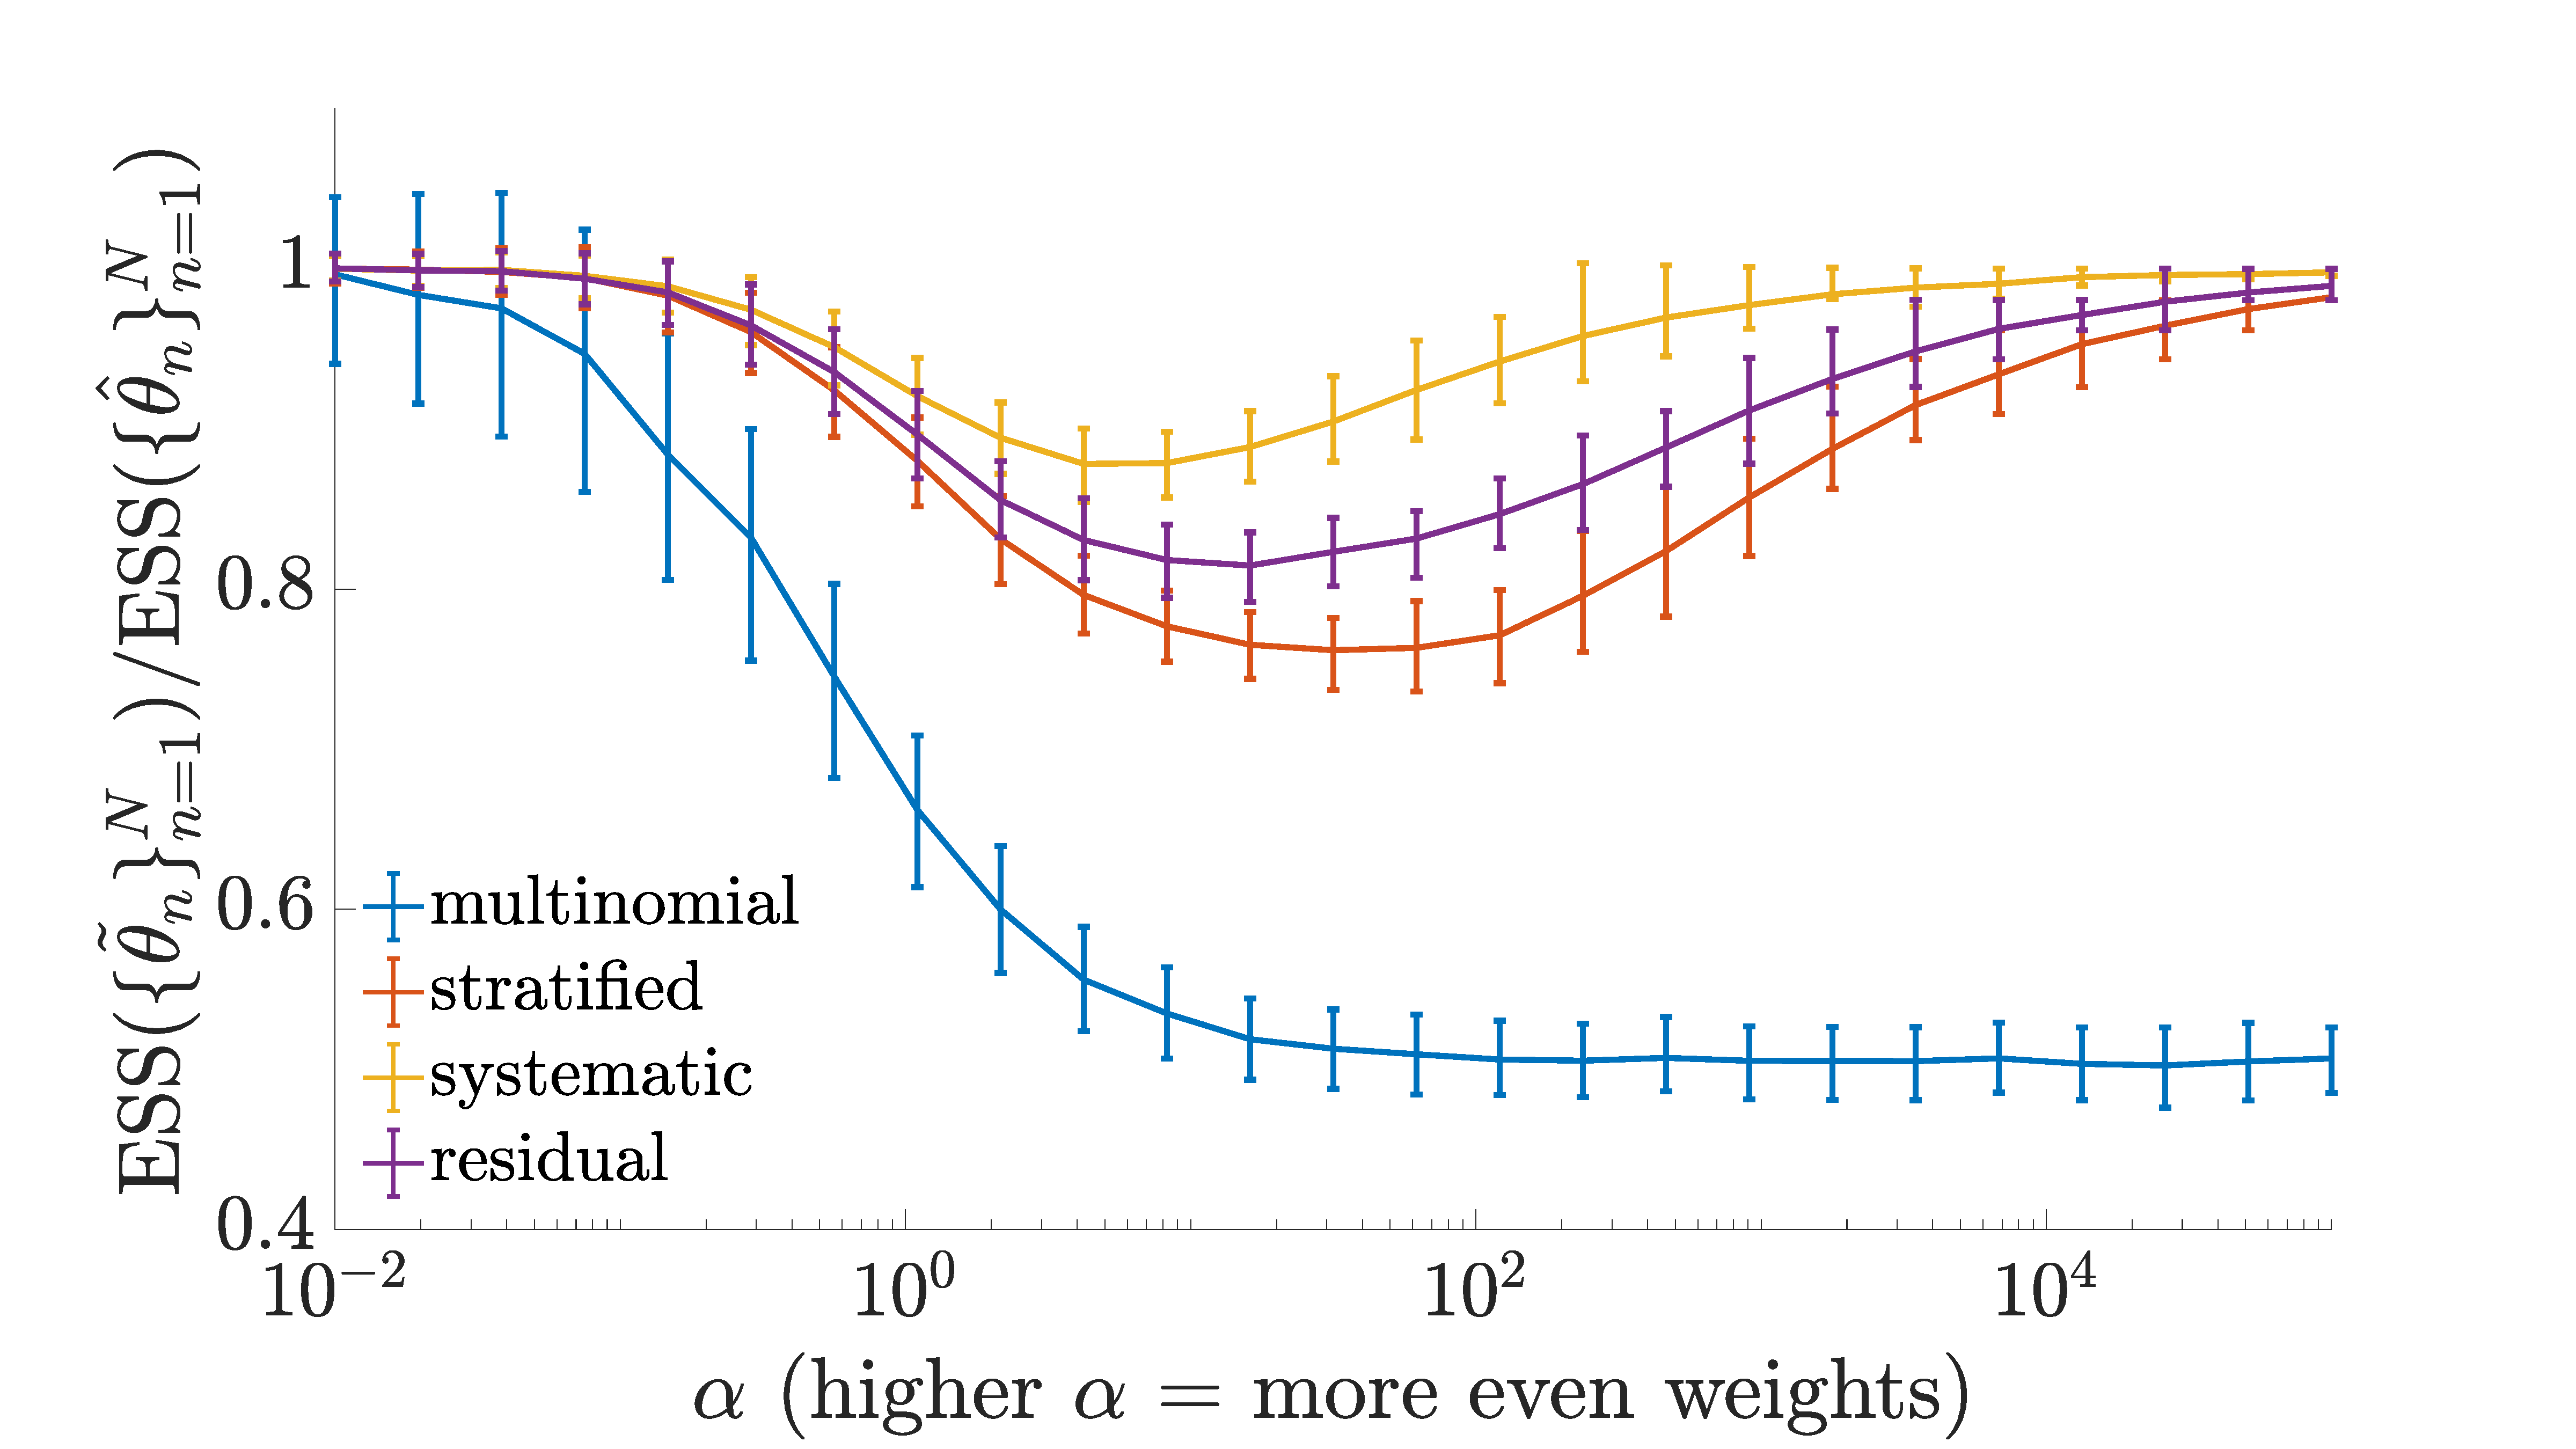
\includegraphics[width=\textwidth]{resampling100}
	\caption{Sample set size $N=100$}
	\end{subfigure}
	~
	\begin{subfigure}[t]{0.49\textwidth}
	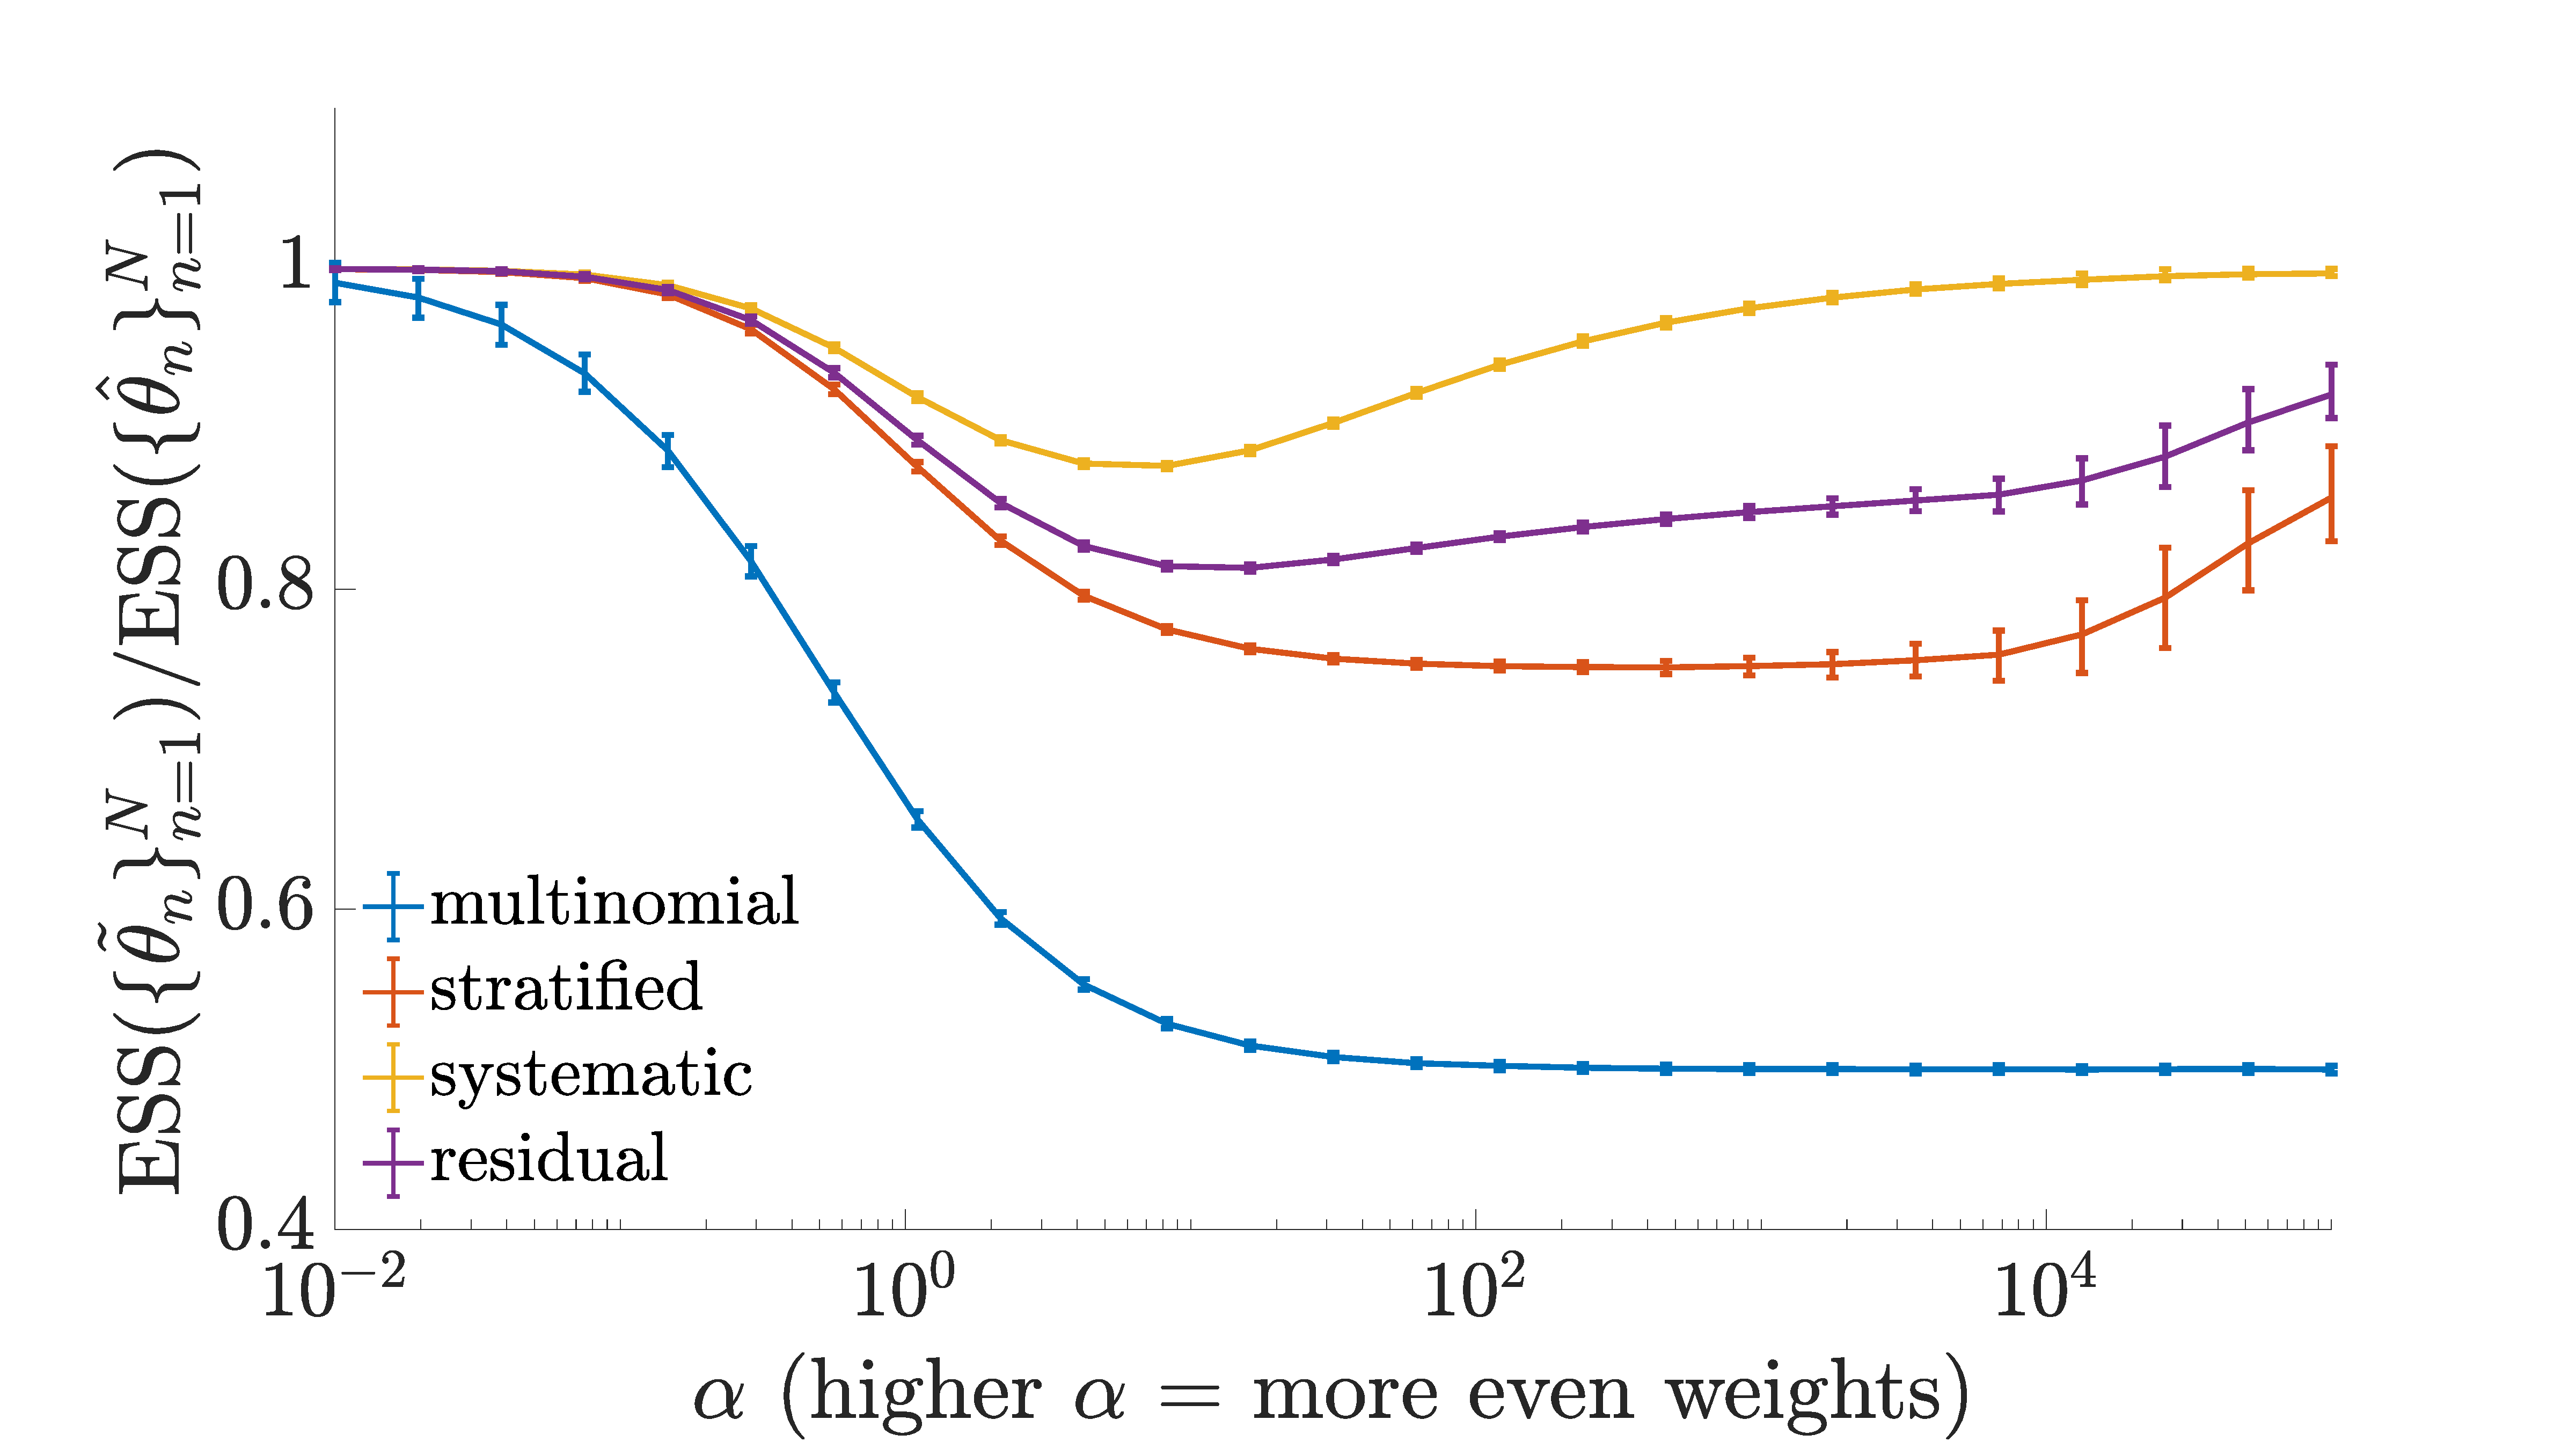
\includegraphics[width=\textwidth]{resampling10000}
	\caption{Sample set size $N=10000$}
	\end{subfigure}
	\caption{Demonstration of performance of different resampling schemes for
		two different sample set sizes and different levels of variance in the weights.
		Plots are generated by first sampling a set of $N$ weights from a symmetric
		Dirichlet distribution with parameter $\alpha$, 
		$\{\bar{w}_n\}_{n=1}^N \sim \textsc{Dirichlet}(\alpha)$, such that the
		higher $\alpha$ is, the more even the weights are on average.  The effective
		sample size (ESS) as defined in~\eqref{eq:inf:ess} is then calculated before an after the
		resampling is carried out, and the ratio of the ESS after to the ESS before
		reported.  Plots show the mean across $1000$ independent trials, with the
		error bars corresponding the to the interquartile range.
		\label{fig:inf:resample}}
\end{figure}

An empirical assessment of the methods is shown in Figure~\ref{fig:inf:resample}.  This shows
the relative effective sample size (ESS) before an after resampling as a function of the uniformity of
the weights.  To calculate the ESS after the resampling, we collapse the identical duplicated
particles down to a single sample with the combined weight of the other samples.  This is equivalent
to replacing $w_n$ with $k_n/N$ in the ESS calculation given in~\eqref{eq:inf:ess}.
Figure~\ref{fig:inf:resample} shows that systematic resampling is clearly preferable to the alternatives, at least
in the terms of the ESS after resampling for this particular problem, with this improvement consistent across the different
sample size sets.  Similar relatives performances are found if one instead uses the proportion of samples that
survive the resampling as a performance metric.
As expected, multinomial resampling is significantly worse than the other
methods, particularly when the weights are more even.  The results also suggest that residual
resampling outperforms stratified resampling, though this can come at the cost of being more
complicated to implement and potentially slower to run.  Note that the reason the ESS sometimes
rises above $1$ for a particular trial is because it is an imperfect measure of the information 
stored in the samples and so this simply happens by chance.
% !TEX root = ../main.tex

\subsection{The Curse of Dimensionality}
\label{sec:inf:foundation:curse}

In this section, we digress from introducing specific inference methods themselves
to talk about a common problem faced by most inference methods, the
\emph{curse of dimensionality}~\citep{bellman1961adaptive}.  At a high-level, the curse of 
dimensionality is a tendency
of modeling and numerical procedures to get substantially harder as the dimensionality increases, 
often at an exponential rate.  If not managed properly, it can cripple the performance of
inference methods and it is the main reason the two procedures discussed so far, rejection
sampling and importance sampling, are in practice only used for very low dimensional problems.
At its core, it stems from an increase of the size (in an informal sense) of a problem as the
dimensionality increases.  This is easiest to see for discrete problems.   Imagine we are calculating
an expectation over a discrete distribution of dimension $D$, where each dimension has $K$
possible values.  The cost of enumerating all the possible combinations scales as $K^D$ and thus
increases exponentially with $D$; even for modest values for $K$ and $D$ this will 
be prohibitively large.

However, the curse of dimensionality extends far beyond problems of enumeration.  It will be felt, to
some degree or another, by almost all approaches for inference and modeling more generally,
but its effect will be most pronounced for methods that try to explicitly model the target
space.  As a geometrical demonstration of this, consider the effect of dimensionality on 
the sampling by rejection approach introduced at the start of Section~\ref{sec:inf:foundation:rejection}.
% where to
%sample uniformly from within some shape we sample uniformly from
%some bounding shape or box containing the target shape and then take only the samples
%that fall within the target.  
For simplicity, we will presume that the target shape is a hypersphere and that
the bounding shape is the smallest hypercube that encloses that hypersphere.  Our acceptance rate,
and thus the efficiency of the algorithm, will be equal to the ratio of the two hyper-volumes.  
For an even number of dimensions,
the hyper-volume of the $D$-dimensional hypersphere with radius $r$ is $V_{s} = \frac{\pi^{D/2}r^D}{(D/2)!}$
and the hyper-volume of the enclosing hypercube is $V_c = (2r)^D$, giving a ratio of
$\frac{V_s}{V_c} = \frac{\pi^{D/2}}{(D/2)! 2^D} = \left(\frac{\sqrt{\pi}}{2}\right)^D\frac{1}{(D/2)!}$.
The first of these terms decreases exponentially and second
super-exponentially with $D$ (noting that $(D/2)!>(D/6)^{(D/2)}$).  
For example, $D=10, 20$, and $100$ respectively gives ratios of approximately
$2.5 \times 10^{-3}$, $2.5 \times 10^{-8}$, and $1.9\times 10^{-70}$.  
Consequently, our acceptance rate will diminish
super-exponentially with the number of dimensions and our approach will quickly become
infeasible in higher dimensions.

An immediate possible criticism of this analysis would be to suggest that the approximation of the
target shape provided by our bounding shape is simply increasingly poor as the dimensionality 
increases and that we should choose 
a better approximation.  Although this is true, the key realization is that achieving a good approximation
is increasingly difficult in high dimensions, typically exponentially so.
To demonstrate this, imagine we instead use an arbitrary bounding shape defined in polar
co-ordinates, such that the proportional difference in the radius at the any given point is at most $\varepsilon$
(i.e. the radius of our bounding shape is between $r$ and $r(1+\varepsilon)$ at all points).
The hyper-volume in which our approximation might live for an even number of dimensions
is given by
\begin{align}
\label{eq:inf:vol-edge}
V_{\varepsilon} = \frac{\pi^{D/2}r^D(1+\varepsilon)^D}{(D/2)!}-\frac{\pi^{D/2}r^D}{(D/2)!}
= V_s \left(\left(1+\varepsilon\right)^D-1\right).
\end{align}
Consequently, we have that the ratio $\frac{V_{\varepsilon}}{V_s}$ increases exponentially with $D$
and that for sufficiently large $D$ and a fixed $\varepsilon$ the amount of space in our tolerance
region will become substantially larger than the target hyper-volume, again leading to very low acceptance
rates.

Flipping this on its head, we can ask the question how does $\varepsilon$ need to vary
to ensure that $V_{\varepsilon}/V_s$ remains constant?  A quick manipulation shows
that $\varepsilon = \left(\left(\frac{V_{\varepsilon}}{V_s}+1\right)^{1/D}-1\right)$ and therefore that
$\frac{\log \left(\frac{V_{\varepsilon}}{V_s}+1\right)}{D} \ge \log(1+\varepsilon) \approx \varepsilon$
for small values of $\varepsilon$.  Thus we only need to decrease $\varepsilon$ roughly
in proportion to $\frac{1}{D}$ to achieve a fixed ratio.  Initially, this would not seem
so bad.  For example, if $D=1000$ we
roughly need $\varepsilon \le 6.9 \times 10^{-4}$ to get $V_{\varepsilon}/V_s \le 1$.
However, this misses the
key difficulty caused by~\eqref{eq:inf:vol-edge}: the higher $D$ is, the more difficult it is
to accurately model the target shape and keep $\varepsilon$ small.  
It follows from~\eqref{eq:inf:vol-edge} that as $D$ increases, the more the hyper-volume
of the sphere is concentrated at the surface.  This generalizes to non-spherical targets and
means that accurate modeling the surface of our target is essential in high dimensions.
Unfortunately, this task becomes rapidly more difficult with increasing dimensionality.  

Consider, for example,
regressing the surface of the target by using a number of inducing points spread over the
surface.  As the dimensionality increases, these become increasingly far apart from one
another and so the more points we need to accurately model the surface.  For example, the
probability of two points uniformly distributed on the surface of a sphere being within
some target distance of one another decreases exponentially
with the dimensionality of the sphere.  This can be seen by noting that a necessary condition
for two points to be within $d$ of each other, is that the discrepancy of each individual dimension 
must be less than $d$.  In other words, if we denote the overall distance as $\delta$ and 
the distance in each dimension as $\delta_i$ then we have 
\[
P(\delta \le d)\le P(\delta_1 \le d)  P(\delta_2 \le d)  \dots  P(\delta_D \le d) 
\]
and so $P(\delta \le d)$ must decrease exponentially with $D$.  
If the correlation between points is proportional to their euclidean distance, then
we will subsequently need an exponentially large number of points in the dimension
to model the surface to a given accuracy.  Consequently, we see that not only are we
increasingly punished for any discrepancies between our approximation and the target
as the dimensionality increases, it rapidly becomes harder to avoid these discrepancies
in the first place.

One can informally think of the proposals we have introduced thus-far as being
approximations to the target distribution: complications with tail behavior aside, it will
generally be the case that the better the proposal approximates the target, the better the
inference will perform.  This typically leads to catastrophically bad performance for
importance sampling and rejection sampling in high dimensions, for which this approximation
breaks down for the reasons we have just outlined.  To give a simple example, imagine that
our target is an isotropic unit Gaussian and we use an independent student-t distribution
with $\nu=2$ in each dimension as the proposal.  We have that the weights are as follows
\begin{align}
w(\theta) = \frac{\pi(\theta)}{q(\theta)} &= \prod_{i=1}^{D} \frac{\exp(-\theta_d^2/2)/\sqrt{2\pi}}
{\frac{\Gamma(1.5)}{\sqrt{2\pi}}\left(1+\theta_d^2/2\right)^{-3/2} } =\prod_{i=1}^{D} \frac{2 \exp(-\theta_d^2/2) \left(1+\theta_d^2/2\right)^{3/2}}{\sqrt{\pi}}.
\end{align}
It follows that the variance of the weights under the proposal increases exponentially
with $D$ as
\begin{align}
\var_{q(\theta)} \left[w(\theta)\right] &= \int w^2(\theta)q(\theta)d\theta -
\left(\int w(\theta)q(\theta)d\theta\right)^2 
=-1+ \prod_{i=1}^{D} \int_{-\infty}^{\infty} w^2(\theta_d)q(\theta_d)d\theta_d \nonumber\\
&=-1+\prod_{i=1}^{D} \int_{-\infty}^{\infty} \frac{\sqrt{2}\exp(-\theta_d^2)\left(1+\theta^2_d/2\right)^{(3/2)}}
{\pi}d\theta_d \approx 1.1455^D-1
\end{align}
where we have used the fact that the integral has a closed form solution.
We thus see that our effective sample size
will drop exponentially quickly with $D$ and that our inference will break down if
the dimensionality is too high.

It is now natural to ask whether we can overcome the curse of dimensionality.  Thankfully, the
answer in many scenarios is that we can.  In many high-dimensional scenarios, the target
distribution will only have significant mass in a small proportion of the total area, often
concentrated around a lower dimensional manifold of the larger space.  This means that if
we use inference methods that in some way exploit the structure of the target distribution and only
search the small subset of the space with significant mass, then effective inference can still be
performed.  When this is not the case, practical inference will typically be futile in high dimensions anyway
and so many inference algorithms are geared towards exploiting a particular type of structure.
As we will show in the next section, the effectiveness of MCMC methods is mostly based on 
exploiting single modality in the target by making local moves that cause the algorithm to have a
hill-climbing style behaviour away from the mode and then sticking close to the mode once it
is found.  Sequential \mc methods on the other hand rely on using the structure of the target
more explicitly, by using a series of stepping-stone distributions and adaptively allocating
resources (see Chapter~\ref{chp:part}).  Variational and message passing methods make assumptions
or approximations about the structure of the model to break the inference problem down
into a number of small problems that can then be combined into an overall estimate.
Arguably the key to all advanced inference methods is how well they can exploit structure
in higher dimensions, while the relative performance of different methods tends to come down
to how suited the target is to their particular form of structure exploitation.
% !TEX root = ../main.tex

\subsection{Markov Chain Monte Carlo}
\label{sec:inf:foundation:mcmc}

\todo[inline]{This section needs quite a bit of cleaning such as transitioning the notation}

Markov chain Monte Carlo (MCMC) methods \cite{metropolis1953equation,hastings1970monte,gilks1995markov} 
form one of the key approaches to circumventing the curse of dimensionality
and are perhaps the most widely used class of algorithms for Bayesian inference, though they
are also used extensively outside the Bayesian inference setting.  The key idea is to construct
a valid Markov chain that has the target distribution as its equilibrium distribution.  They are suitable
for Bayesian inference because this can typically done when the target distribution is only known
up to a normalization constant.  

The reason that they are often able to overcome, or at least alleviate,
the curse of dimensionality is that rather then trying to independently sample from the target distribution
at each iteration, they instead make \emph{local} moves from their current position.  As with
rejection sampling and importance sampling, they use a proposal distribution, but unlike these
alternatives, the proposal is defined conditionally on the current location, namely they propose
according to $x' \sim q(x' | x)$ where $x$ is the current state and $x'$ is the new
state to sample.  The underlying intuition behind this is that in high dimensions the proportion of the
space with significant probability mass is typically very small.  Therefore, if the target is single modal (or
we have a proposal that is carefully designed to jump between modes), then once we have a sample
in the mode, all the other points with significant mass should be close to that point.  Therefore we can
explore the mode by restricting ourselves to local moves, overcoming the curse of dimensionality by
predominantly ignoring the majority of the space as this has insignificant probability mass.  As the
dimensionality increases, the proportion of the space with significant mass decreases, counteracting
many of the other complications that arise from the increasing dimension.  When away from a mode,
they often behave like hill-climbing algorithms, emphasizing their close links with simulated annealing~\citep{aarts1988simulated}
methods for optimization.  Therefore they can be highly effective for both finding the mode
of a posterior and then sticking to that mode.

\subsubsection{Markov Chains}
\label{sec:inf:foundation:mcmc:markov}

We first introduced the concept of the \emph{Markov property} in Section~\ref{sec:bayes:paradigm:graph}
in the concept of a hidden Markov model, where we explained how in Markovian system
is independent of all the previous states given the last state, i.e. 
\begin{align}
\label{eq:inf:markov-prop}
p(X_n = x | X_1 = x_1, \dots, X_{n-1} = x_{n-1}) = p(X_n = x_n  | X_{n-1} = x_{n-1}).
\end{align}
In other words, it transitions from
one state to the next based only on the current state.  Here the series $X_1,\dots,X_n,\dots$ 
is known as a Markov chain.  We see that a probability of a Markov chain is fully defined
by the probability of its initial state $p(X_1 = x_1)$ and the probability of its transitions
$p(X_n = x_n  | X_{n-1} = x_{n-1})$.  If each transition has the same distribution, i.e.
\begin{align}
\label{eq:inf:homo}
p(X_{n+1} = x_{n+1}  | X_{n} = x_{n}) = p(X_{n} = x_{n+1}  | X_{n-1} = x_{n}),
\end{align}
then the Markov chain is known as homogeneous.  Most MCMC methods are based on
homogeneous Markov chains (the exception being adaptive MCMC methods, see Section~\ref{sec:inf:proposal-adapt})
and so we will assume that~\eqref{eq:inf:homo} hold from now on.  In such situations,
$p(X_{n+1} = x_{n+1}  | X_{n} = x_{n})$ is typically known as a \emph{transition kernel}
$T(x_{n+1} \leftarrow x_n)$.

The marginal probability density of any particular point in a homogenous Markov chain is given by
\begin{align}
p(x_n) = \int_{x_1,\dots,x_{n-1}} p(x_1) \prod_{i=2}^{n} T(x_{i=1} \leftarrow x_{i}) dx_1\dots dx_{n-1}.
\end{align}
 For a Markov chain to converge to a target distribution $\pi (x)$, we will need that
$\lim\limits_{n\rightarrow\infty} p(X_n=x) = \pi(x)$ for any possible starting position $x_1$, i.e.
that the chain converges in distribution to the target for all possible starting positions.   For this
to happen we need two things -- $\pi(x)$ must be a \emph{stationary distribution} of the Markov
chain, such that if $p(X_n=x) = \pi(x)$ then $p(X_{n+1}=x) = \pi(x)$, and all possible starting points
$x_1$ must converge to this distribution.  The former of these will be satisfied if 
\begin{align}
\label{eq:inf:stationary}
\pi(x') = \int_{x} T(x' \leftarrow x) \pi(x)dx
\end{align}
where we see that the target distribution is \emph{invariant} under the application of the transition kernel.
Thus if $p(x_n)=\pi(x)$ for some $n$, all subsequent points will have the desired distribution.
The requirement that all starting points converge to the desired target distribution is known
as \emph{ergodicity} which guarantees both the uniqueness of the stationary distribution
and that all points converge to this distribution.  Ergodicity requires that the Markov chain is
\emph{irreducible}, i.e. all points with non-zero probability can be reached in a finite number
of steps, and \emph{aperiodic}, i.e. that no states can only be reached at certain periods of 
time.   We will not delve into the specifics of ergodicity in depth, but note only that homogeneous
Markov chains that satisfy~\eqref{eq:inf:stationary} can be shown to be ergodic under very weak
conditions, see for example~\cite{neal1993probabilistic,tierney1994markov}.

\subsubsection{Detailed Balance}
\label{sec:inf:foundation:mcmc:db}

A common sufficient (but not necessary) condition used for constructing valid Markov chains
is to ensure that the chain satisfies the condition of \emph{detailed balance}.  Chains that
satisfy detailed balance are known as 
\emph{reversible}.\footnote{An interesting area of current research is in the study
	of non-reversible MCMC algorithms~\cite{bouchard2015bouncy,bierkens2016zig}.  These can
	be beneficial because traditional reversible processes are only able to move by drifting over time -- generally
	at least half of the proposed samples (and generally much more) will be in a direction at odds to
	this drift.  By forcing multiple steps in a particular direction before changing the direction can thus
	help  the chain to mix faster.}
For a target $\pi(x)$ then detailed balanced is defined as
\begin{align}
\label{eq:inf:det-bal}
\pi(x) T(x' \leftarrow x) = \pi(x') T(x \leftarrow x').
\end{align}
It is straightforward to see that Markov chains satisfying detailed balance will admit $\pi(x)$
as a stationary distribution by noting that
\begin{align}
\pi(x') &= \int_{x} T(x' \leftarrow x) \pi(x)dx = \pi(x') = \int_{x} T(x \leftarrow x') \pi(x')dx = \pi(x') \\
&= \int_{x} p(x|x') \pi(x')dx = \pi(x') \int_{x} p(x|x') dx = \pi(x')
\end{align}
as required.  Thus any Markov chain we construct that satisfies~\eqref{eq:inf:det-bal}
will converge to the target distribution.  From an inference perspective, this means that
we can eventually generate samples according to our desired target by choosing an 
arbitrary start point $X_1$ and then repeated sampling from our transition kernel $T(X_n \leftarrow X_{n-1})$.

\subsubsection{Metropolis Hastings}
\label{sec:inf:foundation:mcmc:mh}

One of the simplest and most widely used MCMC methods is Metropolis Hastings (MH)~\cite{hastings1970monte}.
Given an unnormalized target $\gamma(x)$, the MH algorithm then at each iteration one samples 
a new point $x'$ according to the a proposal $x' \sim q(x' | x_n)$ conditioned on the current point $x_n$ 
and then accepts the new sample with probability
\begin{align}
\label{eq:inf:accept-prob}
P(\text{Accept}) = \min \left(1, \frac{\gamma(x') q(x_n | x')}{\gamma(x_n) q(x' | x_n)}\right).
\end{align}
At iteration $n$ then we set $x_{n+1} \leftarrow x'$ if the sample is accepted and otherwise
set $x_{n+1} \leftarrow x_{n}$.  Critically this process does not require access to the normalized
target $\pi(x)$.  It is trivial to show that~\eqref{eq:inf:accept-prob} satisfies detailed
balance and therefore produces a valid Markov chain as follows
\begin{align*}
\pi(x_n) T(x_{n+1} \leftarrow x_n) &= \min \left(1, \frac{\gamma(x_{n+1}) q(x_n | x_{n+1})}{\gamma(x_n) q(x_{n+1} | x_n)}\right)
\pi(x_n) q(x_{n+1} | x_n) \\
&= \min \left(\gamma(x_n) q(x_{n+1} | x_n),\gamma(x_{n+1}) q(x_n | x_{n+1})\right) / Z \\
&= \min \left(\frac{\gamma(x_n) q(x_{n+1} | x_n)}{\gamma(x') q(x_n | x_{n+1})},1\right) \pi(x_{n+1}) q(x_n | x_{n+1}) \\
&=\pi(x_{n+1}) T(x_n \leftarrow x_{n+1}),
\end{align*}
as required.

Though MH is valid for any reasonable choice of the proposal distribution\todo{Be more specific},
the practical performance will depend heavily on the choice of the proposal $q(x'|x)$.
For example, if $q(x'|x)$ is independent of $x$ then no information is passed from one iteration
to the next and gives and one gets an algorithm that is strictly worse than importance sampling
because samples are independently generated in the same way, but information is lost in the accept-reject
step.  Instead, one will generally want to propose points close to the current point so the advantages
of \emph{local moves} can be exploited.  However, this has complications as explained in the next
section, while choosing the a proposal with the right characteristics is still rather challenging.
For example, image we use an isotropic Gaussian proposal, corresponding to a random walk without the
accept reject step.  If the variance of our proposal is too high then we will rarely propose good points
and so the acceptance rate will become very low, giving few distinct samples.  If the variance is too low,
the Markov chain will move very slowly as it can only take small steps.  This will increase correlation
between all our samples and reduce the fidelity of our estimates.  Chain that quickly cover the full
probability space are said to \emph{mix} quickly.

\subsubsection{Intuitions, Complications, and Practical Considerations}
\label{sec:inf:foundation:mcmc:intuitions}

Though MCMC methods can be exceptionally effective, they are not without their weaknesses.
Most of these weakness stem from the fact that all the generated samples are correlated, leading to, for
example, biased estimates.  Clearly this reduces the amount of distinct information conveyed by 
each sample and this will reduce the accuracy of the estimator.  However, it also causes more fundamental
issues.
Most of the convergence results we have presented so far have relied on samples being generated in a i.i.d. 
fashion which is clearly not the case in the MCMC setting.  MCMC methods therefore require their own
unique convergence proofs, based in general on ergodic theory.
\todo[inline]{Add these, e.g. Birkhoff Ergodic Theorem,
	pointwise ergodic theorem.  Probably worth its own section or a least a paragraph to talk about the
	requirements for ergodicity} 

These convergence results show that the bias of MCMC tends to zero
as the number of iterations tends to infinity, but it is often very difficult to magnitude of the bias for
finite numbers of iterations.  Whereas importance sampling and rejection sampling had reasonable
diagnostics for the performance of the inference, such as the effective sample size and the acceptance
rate respectively, estimating the bias from MCMC samplers is typically fiendishly difficult and it can
often look like an MCMC sampler is performing well (e.g. in terms of its acceptance rate) when in fact it is doing disastrously.  
One of the most common ways this is manifested is in the sampler becoming stuck in a particular 
mode of the target.  If a target has more than a single mode then using localized proposals can make
it prohibitively difficult to move between the modes.  Though convergent MCMC samplers must eventually
visit every mode infinitely often, it can take arbitrarily long to even visit each mode once.  Even worse,
getting the correct estimate relies on spending the correct relative proportion of time in each mode which
will typically take many orders of magnitude more time to get an reasonable estimate for than just to
have the sampler visit each significant mode at least once.  The issues associated with multiple modes
provides a demonstration of why it is difficult to estimate the bias of an MCMC sampler: we do not in
generally know or are even able to provide reasonable estimates for if we have missed another mode or 
whether our sampler has spent an appropriate amount of time in different modes.

Because of these drawbacks, MCMC is rarely used on multi-modal problems unless an appropriate mechanism
for transitioning between the modes can be found.  Thankfully, many problems become increasingly single-modal
in high dimensions CITE SOMETHING and so there are a surprisingly wide array of models that actually 
fit these restrictions, particularly if we can find an appropriate parameterization of the model.  Remembering
from section~\ref{sec:prob:measure} that changing the parameterization of a model changes its probability
density function in a non-trivial manner, the performance of MCMC methods is often critically dependent on
their parameterization.  There are two effects at play here. Firstly changing the parameterization will change
the concept of what parameter values are close to which other parameter values.  In an ideal world we
would make moves in the raw sample space where all points are equally probable before calculating the
random variables from the position in sample space.  Typically this is not practical, but it is still usually the
case that some parameterizations will tend to be more single-modal and more generally have all points of
interest close together in the parameter space.  Note that there is often an equivalence here between a good proposal,
and a good warping of the space to one where an isotropic proposal will be effective.  

Secondly, higher dimensional parameterizations are less likely to become stuck in a local mode.\todo{Need some citations}
At a high level, the more variables that can be changed to some significant effect, the less likely that
it is detrimental to change any one of the variables.  In essence, projecting into a higher dimensional
space provides more degrees of freedom for changes in the proposal and this helps to keep the Markov
chain moving and to make distinct moves at each iteration.  Though somewhat counter intuitive, projecting
to higher dimensional spaces is key to a number of MCMC samplers performing effectively.\todo{Add examples}

Unfortunately MCMC does not provide natural or unbiased estimates for the marginal likelihood in
the same manner as importance sampling or rejection sampling ...

\subsubsection{Gibbs Sampling}
\label{sec:inf:foundation:gibbs}

Gibbs sampling is an important special case of Metropolis-Hastings that looks to update only some
subset of variables in a joint distribution.  Imagine we have target $D$ distributional target distribution
$\pi(\theta)$ where $\theta = \{\theta_1,\theta_2,\dots,\theta_D\}$.  Gibbs sampling incrementally
updates one or more of the variables $\theta_d$ at each iteration conditioned on the value of the others.
Thus it uses proposals of the form $\theta_d' \sim \pi(\theta_d' | \theta \backslash \theta_d)$ with
$ \theta \backslash \theta_d$ kept constant from one iteration to the next.  There are two reasons
for wanting to do this.  Firstly changing only of the variables at a time is a form of local proposal and
can be a beneficial way to make updates, particularly if random walk proposal are inappropriate, for example
because the variables are not continuous.  Secondly, if we have access to $\pi(\theta_d | \theta \backslash \theta_d)$
exactly, then we will actually accept every sample as
\begin{align*}
\frac{\pi(\theta)\pi(\theta_d' | \theta \backslash \theta_d)}{\pi(\theta')\pi(\theta_d | \theta' \backslash \theta_d')}
&=\frac{\pi(\theta_d |  \theta \backslash \theta_d) \pi( \theta \backslash \theta_d)
	\pi(\theta_d' | \theta \backslash \theta_d)}
{\pi(\theta_d' |  \theta' \backslash \theta_d') \pi( \theta' \backslash \theta_d')\pi(\theta_d | \theta' \backslash \theta_d')} \\
\intertext{now noting that $\theta' \backslash \theta_d' = \theta \backslash \theta_d$}
&=\frac{\pi(\theta_d |  \theta \backslash \theta_d) \pi( \theta \backslash \theta_d)
	\pi(\theta_d' | \theta \backslash \theta_d)}
{\pi(\theta_d' |  \theta \backslash \theta_d) \pi( \theta \backslash \theta_d)\pi(\theta_d | \theta \backslash \theta_d)} 
= 1.
\end{align*}
In many models it will be possible to sample from $\theta_d' \sim \pi(\theta_d' | \theta \backslash \theta_d)$
exactly\todo{give examples} and thus carry out Gibbs sampling exactly.  We can then cycle through each of
the $\theta_d$, either in a random order or in sequence, and apply the appropriate updates.  The
effectiveness of this approach will depend on the level of correlation between the different variables.  The more
correlated each variable: the smaller the updates will be for each variable conditioned on the values of the
others and the slower the chain will mix.  In extreme cases, this does impose stricter conditions
for convergence for Gibbs samplers than MH~\citep{roberts1994simple}.  For example, consider an exclusive
or style problem where $\pi(\theta_1,\theta_2) = 1$ if $0\le\theta_1\le1$ and $0\le\theta_2\le1$
or $-1\le\theta_1<0$ and $-1\le\theta_2<0$ and $\pi(\theta_1,\theta_2) = 0$ otherwise.  Here there is no
way to move from the $[0,1]^2$ square to the $[-1,0]^2$ by updating only one of the variables at a time.  As
such a Gibbs sampler would end up stuck in either the positive or negative square.

If it is not possible to sample from the conditional distributions exactly or if it is only
possible for some of the variables, we can instead use a \emph{Metropolis-within-Gibbs} approach,
also known as \emph{component-wise Metropolis-Hastings}, where
we use a proposal to approximate one or more $\pi(\theta_d' | \theta \backslash \theta_d)$ with an
appropriate proposal.  Naturally this means that the acceptance ratio is no longer always $1$ and so
an accept-reject step becomes necessary.  Though the convergence of this approach has
been shown by~\cite{jones2014convergence}, additional assumptions are required compared to the
standard Gibbs or MH cases.

\subsubsection{Advanced MCMC Algorithms}
\label{sec:inf:foundation:advanced}

\todo[inline]{Write me}

\begin{itemize}
	\item HMC and typical distance from mode in high dimensional Gaussian
	\item Slice sampling?
	\item Estimating the normalization constant
\end{itemize}

\subsection{Proposal Adaptation}
\label{sec:inf:proposal-adapt}

\section{Alternatives to Monte Carlo Inference}
\label{sec:inf:alt}

Though our focus in this chapter has mostly been on Monte Carlo inference methods, we finish
by noting that these are far from the only viable approaches.  Two key advantages of Monte Carlo
methods are their ubiquitous nature, i.e. many can almost always be applied, 
and that most commonly used Monte Carlo methods are asymptotically exact, such that given
enough time, we can always achieve a required level of accuracy.  However, in some scenarios,
Monte Carlo methods can be problematically slow to converge and so alternative, asymptotically approximate,
methods can be preferable such as variational inference~\citep{blei2016variational} and
 messaging passing methods~\citep{lauritzen1988local}.  Of these, variational inference has become an increasingly
 popular approach.  Its key idea is to reformulate the inference problem to 
an optimization, by learning parameters of an approximation to the posterior.  Typically this involves
defining some family  of distributions within which the posterior approximation can live, e.g. an exponential
distribution family, and then optimizing an \emph{evidence lower bound} (ELBO) with respect to the parameters of
this approximation.  Doing this implicitly minimizes
the Kullback-Leiber divergence between the approximation the target.
Variational inference often forms a highly efficient means of calculating a posterior approximation, but,
in addition to the obvious bias from using a particular family of distributions for the approximation, it typically
requires strong structural assumptions to be made about the form of the posterior. Namely most methods make a
so-called \emph{mean-field} assumption that presumes that the posterior factorizes over all
latent variables.  Its effectiveness is thus critically dependent on the reasonableness of these assumptions.

